\documentclass[type=bachelor]{thuthesis}
% 选项:
%   type=[bachelor|master|doctor|postdoctor], % 必选
%   secret,                                   % 可选
%   pifootnote,                               % 可选(建议打开)
%   openany|openright,                        % 可选,基本不用
%   arial,                                    % 可选,基本不用
%   arialtoc,                                 % 可选,基本不用
%   arialtitle                                % 可选,基本不用

% 所有其它可能用到的包都统一放到这里了,可以根据自己的实际添加或者删除。
\usepackage{thuthesis}

% 定义所有的图片文件在 figures 子目录下
\graphicspath{{figures/}}

% 可以在这里修改配置文件中的定义。导言区可以使用中文。
% \def\myname{薛瑞尼}

\begin{document}

%%% 封面部分
\frontmatter
\thusetup{
  %******************************
  % 注意:
  %   1. 配置里面不要出现空行
  %   2. 不需要的配置信息可以删除
  %******************************
  %
  %=====
  % 秘级
  %=====
  secretlevel={秘密},
  secretyear={10},
  %
  %=========
  % 中文信息
  %=========
  ctitle={基于B/S与C/S混合架构的行政管理系统},
  cdegree={工学学士},
  cdepartment={计算机科学与技术系},
  cmajor={计算机科学与技术},
  cauthor={滕爽},
  csupervisor={张小平老师},
  %cassosupervisor={陈文光教授}, % 副指导老师
  %ccosupervisor={某某某教授}, % 联合指导老师
  % 日期自动使用当前时间,若需指定按如下方式修改:
  % cdate={超新星纪元},
  %
  % 博士后专有部分
  cfirstdiscipline={计算机科学与技术},
  cseconddiscipline={系统结构},
  postdoctordate={2009年7月——2011年7月},
  id={编号}, % 可以留空: id={},
  udc={UDC}, % 可以留空
  catalognumber={分类号}, % 可以留空
  %
  %=========
  % 英文信息
  %=========
  etitle={An Administrative Management System Based on Mixed B/S and C/S Architecture},
  % 这块比较复杂,需要分情况讨论:
  % 1. 学术型硕士
  %    edegree:必须为Master of Arts或Master of Science(注意大小写)
  %             “哲学、文学、历史学、法学、教育学、艺术学门类,公共管理学科
  %              填写Master of Arts,其它填写Master of Science”
  %    emajor:“获得一级学科授权的学科填写一级学科名称,其它填写二级学科名称”
  % 2. 专业型硕士
  %    edegree:“填写专业学位英文名称全称”
  %    emajor:“工程硕士填写工程领域,其它专业学位不填写此项”
  % 3. 学术型博士
  %    edegree:Doctor of Philosophy(注意大小写)
  %    emajor:“获得一级学科授权的学科填写一级学科名称,其它填写二级学科名称”
  % 4. 专业型博士
  %    edegree:“填写专业学位英文名称全称”
  %    emajor:不填写此项
  edegree={Bachelor of Engineering},
  emajor={Computer Science and Technology},
  eauthor={Teng Shuang},
  esupervisor={Professor Zhang Xiaoping},
  % 日期自动生成,若需指定按如下方式修改:
  % edate={December, 2005}
  %
  % 关键词用“英文逗号”分割
  ckeywords={软件系统, 工程架构},
  ekeywords={Software System, Engineering Architecture}
}

% 定义中英文摘要和关键字
\begin{cabstract}
  
  得益于互联网的发展,现在越来越多的行政管理系统采取了无纸化操作的模式。借由互联网的便利性、实时性、安全性和可靠性作为保证,越来越多的行政工作可以在互联网上高效而自动化地进行,并将统计数据以简洁而又精确的形式,通过数据可视化方法直观地呈现。

  得益于智能手机的普及,互联网系统也逐渐向着移动设备靠拢。结合微信或者手机应用这些成熟的开发平台,即使不在电脑旁边,用户也可以及时地收到最新的新闻资讯或者消息通知。

  目前清华大学的公会暂时没有采用无纸化办公的流程。活动发布、人员管理和签到记录暂时还基于传统的工作模式开展进行。基于这个背景,结合清华大学的公会管理流程,本文将提出一个完整的清华大学公会管理系统架构,并给出其实现,与其他的在线行政管理系统进行对比。

  本文的技术重点主要有:
  \begin{itemize}
    \item 利用AngularJS单一页面应用程序的开发特性及其MVC框架,优化数据传输、页面显示和可拆装性;
    \item 使用RSA加密算法在HTTP协议下仍能保证数据安全;
    \item 基于REST的前后端分离技术,使得一套后端能够服务于复数个前端,增加开发灵活性和可扩展性;
    \item 微信平台的灵活运用,解决了活动消息通知的“最后一公里”问题。
  \end{itemize}

  本文将通过引言、现有工作介绍和对比、系统架构、技术难点、系统展示和结论几个方面,来对清华大学工会管理系统进行详细介绍。

\end{cabstract}

% 如果习惯关键字跟在摘要文字后面,可以用直接命令来设置,如下:
% \ckeywords{\TeX, \LaTeX, CJK, 模板, 论文}

\begin{eabstract}
   
  Thanks to the development of the Internet, more and more administrative system tends to take a paperless mode of operation. As a guarantee, more efficient and automate administrative tasks can be carried out by the convenience of the Internet, real-time, security, and reliability on the Internet, with the statistical data be presented by data visualization methods in a concise and precise form.

  With the prevail of smartphones, the Internet system is also gradually move closer toward mobile devices. Combining with mature development platform like WeChat mobile applications, users can timely receive the latest news or message notification even if they are not next to the computer.

  Currently, the Union in Tsinghua University is not utilizing the Internet facility. Publishing activities, personnel management and attendance records are yet based on the traditional mode of operation. Based on this situation, combined with Tsinghua Union management process, this paper will present a fully functional Tsinghua Union management system architecture and its implementation with a compare with previous works.

  Technical focus of this paper are:  
\begin{itemize}
    \item Use AngularJS single page development features and MVC application framework, to optimize data transmission, display and dismantling of the page;
    \item Using the RSA encryption algorithm in the HTTP protocol to ensure data security;
    \item REST-based technology separates front and back ends, making a backend capable of servicing a plurality of front-end, increase development flexibility and scalability;
    \item Flexible use of WeChat platform, to solve the \"last kilometer\" challenge of message notification issues.
\end{itemize}


\end{eabstract}

% \ekeywords{\TeX, \LaTeX, CJK, template, thesis}

% 如果使用授权说明扫描页,将可选参数中指定为扫描得到的 PDF 文件名,例如:
% \makecover[scan-auth.pdf]
\makecover

%% 目录
\tableofcontents

%% 符号对照表
%\input{data/denotation}


%%% 正文部分
\mainmatter

\chapter{引言}

得益于互联网的发展,现在越来越多的行政管理系统采取了无纸化操作的模式。借由互联网的便利性、实时性、安全性和可靠性作为保证,越来越多的工作可以在互联网上方便地进行。以清华大学的互联网系统为例,清华大学已经拥有了完整成体系的清华大学信息门户系统。辅以清华大学网络学堂,清华大学在线图书馆,清华学生生活,清华大学学业门户,清华大学在线选课系统,清华大学的在线系统已经成相当规模,为师生的学习生活带来了便利,使得学生们可以足不出户地处理各项学习生活服务。就在最近两年,清华大学的自助注册系统上线,更进一步简化了学生注册的步骤。利用互联网技术进行自助服务已经成为了清华大学各项工作改革的主流趋势。

随着Web2.0乃至Web3.0的发展,网页不再是单向向用户传播信息的工具。借由一套基于浏览器的管理系统,用户现在可以通过浏览器向服务器发送控制和命令,以达到管理的目的。这伴随着浏览器的功能逐渐完善,以及得益于W3C组织对浏览器进行标准化的工作,区别于传统的基于客户端的C/S架构的基于浏览器的B/S架构正变得越来越流行。基于B/S架构的行政系统可以脱离一个独立的客户端,直接以网页的形式在网页浏览器中进行原来需要一个独立的客户端才能进行的工作。

另一方面,随着智能手机的不断普及,移动平台的应用也越来越成熟。随着微信开放开发环境的成熟,比起自行开发一个应用,越来越多的企业和学校服务开始倾向于选择微信微平台作为提供服务的平台。这保证了这些服务在提供服务的同时,保证了用户在使用服务时同时能享受到微信方便成熟的社交功能。统一的界面也免去了用户学习应用使用方法的过程,也免去了二次验证和用户账户管理的繁琐,因此出现了这种新兴的C/S架构,即将微信作为自己的C/S,与微信内嵌的浏览器结合,形成B/S和C/S混合架构来提供更完整的服务。

目前,清华大学校内还有许多行政进程没有进行无纸化互联网转变。清华大学校内的工会,暂时还在使用传统人工的方式进行活动发布、人员管理和签到记录。使用这种传统方式进行的方法,既影响了工会工作的效率,又有可能会导致资料丢失和错误,为未来的工作带来不必要的麻烦。

实际上,清华大学工会可以采用一套基于互联网的行政管理系统来统一管理这一系列的流程。本文就将以清华大学的工会管理系统为例,呈现一套完整的基于B/S和C/S混合架构的清华大学工会管理系统的详细架构,具体实现,并和现有的行政系统进行对比,对结论进行阐释。

\chapter{相关工作}

目前已经有相当一部分的互联网行政管理系统的实现\cite{oyj2006}\cite{zw2015}\cite{ysy2000}\cite{wq2010}\cite{sj2004}\cite{hk2013},其中不乏与本文中同样属于工会管理系统的实现案例\cite{hzj2007}\cite{whx2006}\cite{dxl2007}\cite{lzq2010}。然而这些工作\cite{wq2010}\cite{hzj2007}在鼓吹B/S相对于C/S的优越性的时候,却忽略了移动设备上微平台(例如微信)对C/S架构发展的贡献。同时,这些系统往往更多在考虑和介绍自己的针对自己需求的实现,系统存在局限性,无法将设计模式向其他的系统进行外推。更严重的是,这些系统对网络传输的安全性鲜有考虑。对于用户的数据来说,这样的行为是不负责任并且是十分危险的。

也有许多的工会系统是基于微信移动平台进行开发的。其中不乏有将微信开发平台运用在工会系统上的实现\cite{lih2015}。然而这项工作却缺少对技术细节的详细叙述,并且仅仅使用了微信平台作为唯一的信息发布渠道。实际上,碍于移动设备的输入方式受到限制,在微信上进行含有具体内容的信息的发布效率并不高。因此单纯的微信平台会导致信息发布存在障碍,这项工作需要一个基于浏览器的控制端才能高效地运作。其他一些在微信开发平台上的实现\cite{fanfl2013}\cite{qinjj2015}则与行政系统的需求差距比较远,无法适用于本文中系统使用的环境当中,但是其中的使用微信开发的思想却是值得借鉴的。

参考这些现有工作的实现,并结合这些工作中的优点,对其中的缺点进行分析之后,我们可以从中抽象出一套适用于清华大学工会管理系统的系统架构。


\chapter{系统架构}

\section{需求分析}

\label{requireAnalysis}

对于一个行政管理系统而言,最首要的工作是要确定需求。在进行系统架构的设计之前,我们和清华大学工会负责人讨论确定了系统的需求。

图\ref{fig:demand}展示了我们整理的工会管理系统需要实现的功能流程图。

\begin{figure}[H]
  \centering
  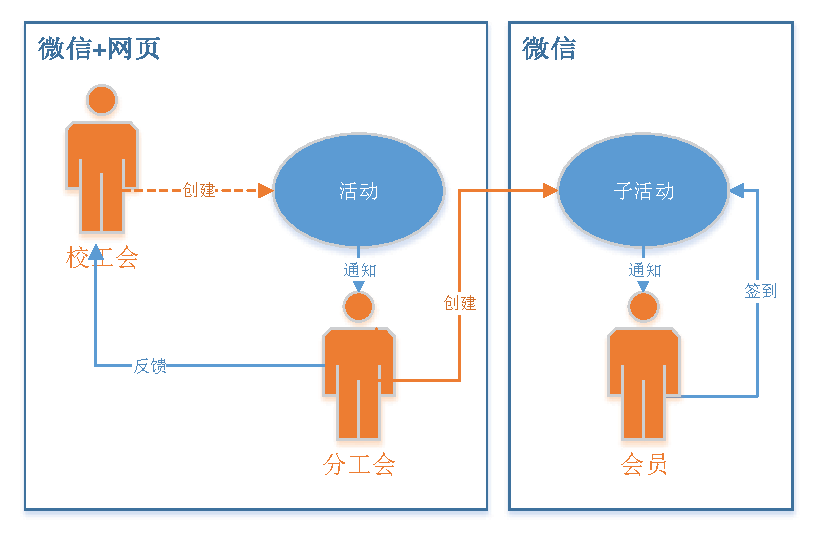
\includegraphics{demand}
  \caption{工会管理系统总体需求流程图}
  \label{fig:demand}
\end{figure}

由需求图中可以看到,整个工会行政过程分为六个主体部分:总工会发起活动,分工会反馈,授权人指定,子活动创建,子活动追踪,以及生成活动报告。通过进一步对需求进行分析可以发现,在工会的管理过程中涉及到三个角色:校工会,分工会和会员。这三种角色的具体职责如图\ref{fig:demand2}所示。

\begin{figure}[H]
  \centering
  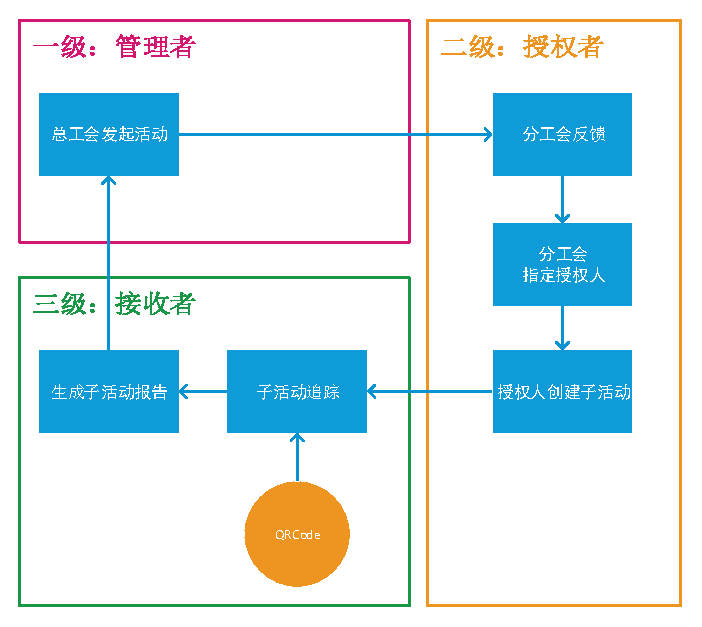
\includegraphics{demand2}
  \caption{工会行政中三种角色及其职责分析}
  \label{fig:demand2}
\end{figure}

更具体的,各个角色的职责可以描述为:

\begin{itemize}
	\item 校工会主席:负责创建一个活动,向分工会主席进行通知并接受一个活动的反馈报告信息;
	\item 分工会主席:负责接收校工会创建的活动,针对活动的要求创建对应的子活动,并将子活动的进行结果制成报告反馈回校工会;
	\item 工会会员:接收子活动推送,参加活动并参与签到。
\end{itemize}

在完成了这些需求的分析和角色的划分之后,就能够开始进行对系统架构的设计和实现工作了。

\section{B/S和C/S混合框架}

正如标题中所言,本文中的系统采用的是B/S和C/S混合系统。B/S架构使用的是浏览器/服务器结构,而C/S架构指的是客户端和服务器结构。即在使用系统的时候,一套Server需要服务两套客户前端。图\ref{fig:overallArchitecture}是一个系统的总体框架示意图,展示了B/S和C/S架构在本文中的系统中的关系。

\begin{figure}[H]
  \centering
  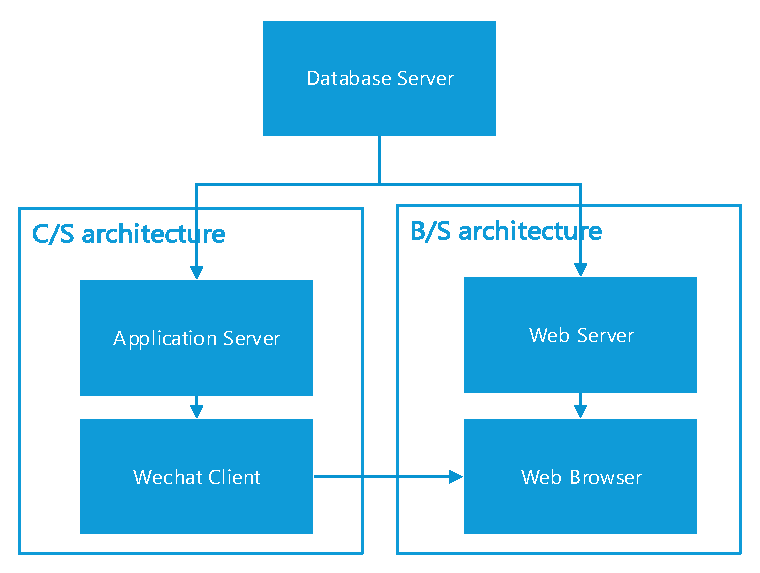
\includegraphics{overallArchitecture}
  \caption{系统的B/S和C/S混合框架}
  \label{fig:overallArchitecture}
\end{figure}

这样设计的原因是借助了桌面平台能够高效率地进行输入工作,并且输入工作对移动性的需求并不高,能够使用浏览器实现跨平台和设备无关就已经能够满足信息的录入对移动便携的需求。另一方面,对于工会活动信息的接收者来说,他们需要随时随地地接收到工会的推送活动消息。目前的浏览器并不能支持实时的消息推送。要实现这一步,需要通过一个浏览器,即本例中的微信企业号微平台,来实现这一步。

其中一个客户前端是传统B/S架构中的Brower角色,即浏览器。用浏览器代替传统的桌面计算机设备上的应用程序,使得系统能够原生地利用浏览器的跨平台特性从而实现跨平台的效果。即无论是在Windows操作系统中还是在OSX操作系统,都可以通过浏览器访问到系统的浏览器客户端,并对系统进行控制和管理。在本文中实现的系统中,甚至实现了可以在手机的浏览器上访问浏览器客户端的内容,实现了高度的兼容性。

另一方面,系统架构中的C/S架构部分则区别于传统的C/S架构。它并不是基于一个独立的移动端应用程序,而是作为微信客户端中“企业号”功能中的一个子项目微平台存在。区别于B/S架构中的浏览器成分,微信中的微平台能够提供浏览器所没有办法提供的推送功能,相当于一个小型的客户端程序。在这样一个麻雀虽小五脏俱全的微型客户端中,结合微信提供的内置浏览器和二维码扫描功能,能够实现包括查看、接收和管理活动的同时,还能进行网页浏览器无法进行的二维码签到功能。

\section{系统架构}

由于系统涉及到两个独立的前端,因此一个解决方法是参考REST架构,将前后端的设计进行分离。如图\ref{fig:architecture}是本系统架构的示意图。

\begin{figure}[H]
  \centering
  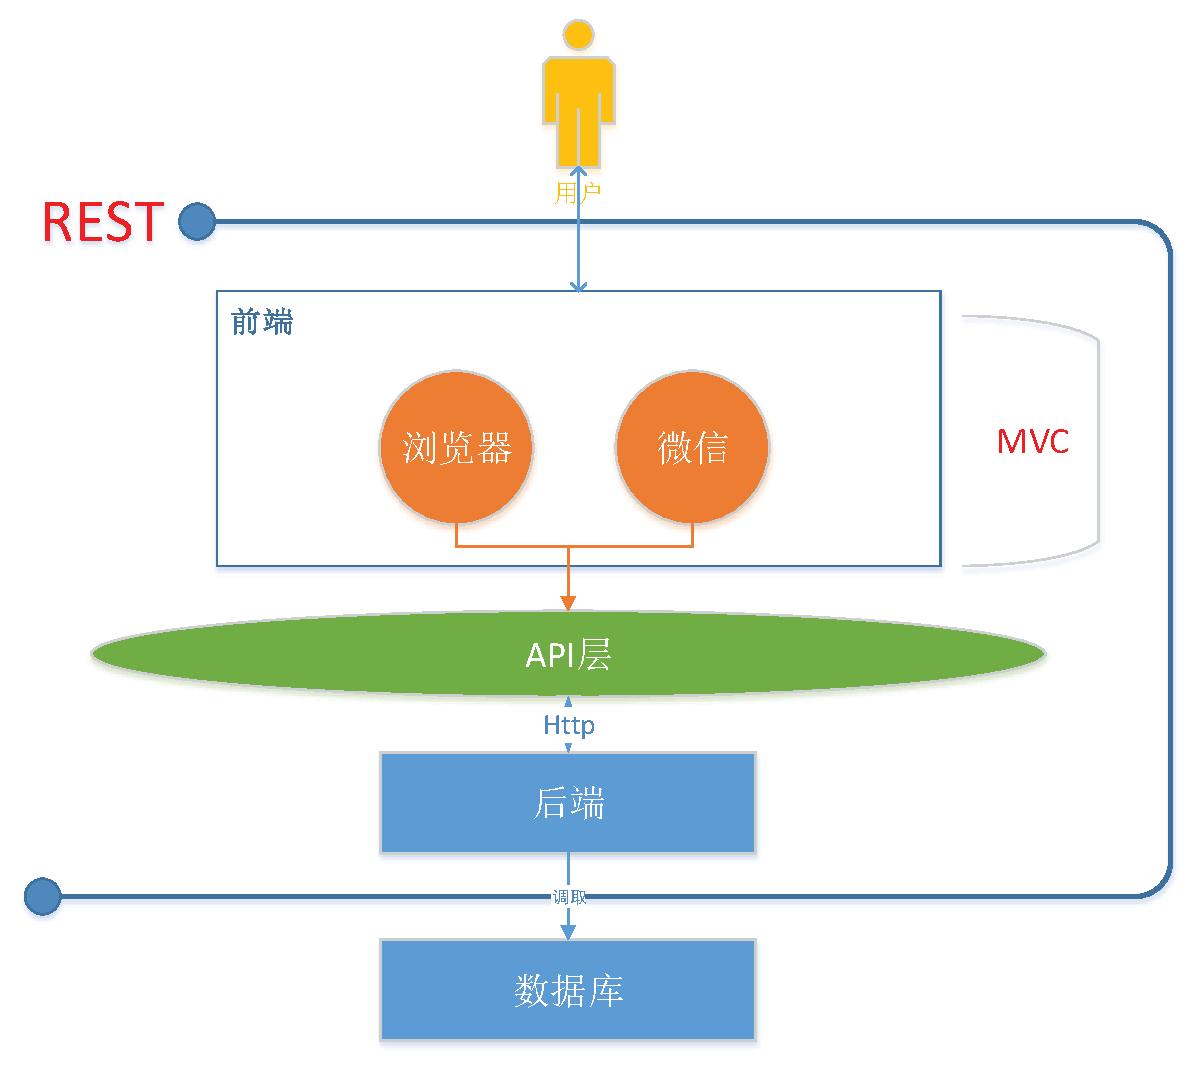
\includegraphics[width=0.8\textwidth]{architecture}
  \caption{系统架构示意图}
  \label{fig:architecture}
\end{figure}

下面将分成前端架构、后端架构和前后端通信三个部分分别对架构进行具体的描述。

\subsection{前端架构}

凭借AngularJS的强大功能,极大地简化了在前端进行网页应用程序开发的过程,并使得前端也能够拥有原来只有在后端才能够实现的MVC架构。前端架构如图\ref{fig:frontMVC}所示。

\begin{figure}[H]
  \centering
  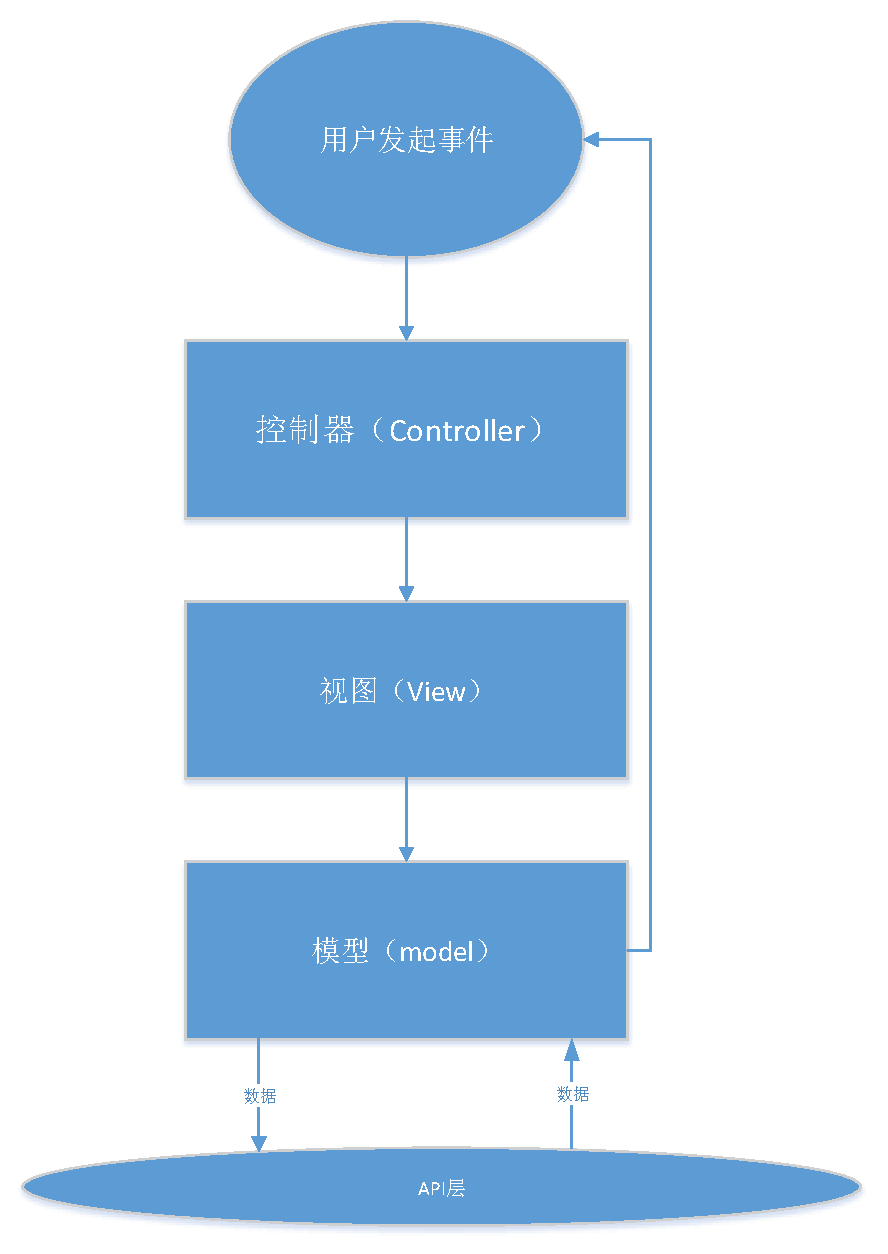
\includegraphics[width=0.5\textwidth]{frontMVC}
  \caption{前端MVC架构示意图}
  \label{fig:frontMVC}
\end{figure}

由前端的控制器接受并响应用户事件,控制视图对页面上对应的元素进行修改,并由视图访问模型元件对API进行调用的过程。由一些具有树状关系的控制器控制多个视图对不同的事件进行响应,同时控制器控制不同的模型对不同的API进行数据的调用和读取请求,使得后端能够对前端的事件作出不同的相应。

在前端使用MVC架构使得前端能够在不刷新页面的情况下,仅仅通过切换视图就可以达到展现不同页面的效果,同时保证了前端数据的去耦合。以MVC架构作为前端设计的页面,规避了Javascript长久以来受人诟病的代码凌乱问题,使得各个部分的代码各司其职,方便模块化进行维护,同时也提供了高度的可拆装性。

有关AngularJS的具体描述,将在\ref{angularJS}节进行详细展开。

\subsection{后端架构}

后端使用了JAVA Servlet作为后端服务器,以Apache Tomcat作为运行环境。由于使用了REST架构,因此后端不涉及数据的显示工作,因此主要包含了四个部分:功能类、数据模型类、Bean类和API类。四个类的具体描述如下:

\begin{itemize}
	\item 功能类:提供与HTTP请求数据无关的功能方法;
	\item 数据模型类:与数据库进行直接通讯的类,将各种对数据库的操作进行封装,使得API类能够通过调用数据模型类的方法可以间接方便地对数据库进行处理;
	\item Bean类:对数据表中的数据格式进行封装,使得API类能够通过JAVA的方式对数据库中的数据进行处理;
	\item API类:唯一的接受HTTP请求并对HTTP请求进行回应的类。
\end{itemize}

更具体的,后端架构如图\ref{fig:backend}所示。

\begin{figure}[H]
  \centering
  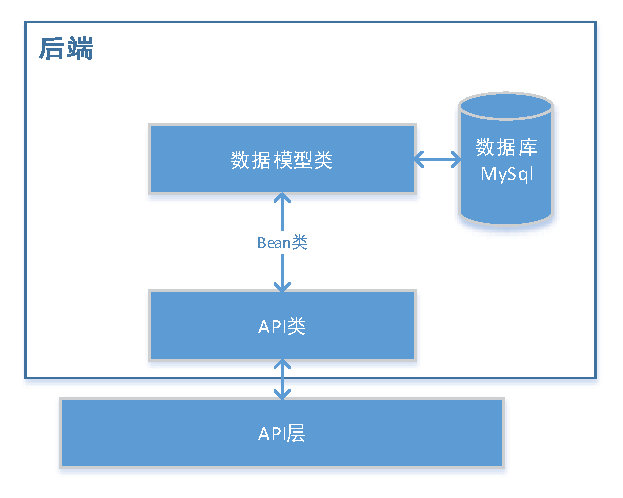
\includegraphics{backend}
  \caption{后端架构示意图}
  \label{fig:backend}
\end{figure}

通过这样的设计能够使得在设计API的过程中无需考虑对数据库的处理,而设计数据模型类的时候,也可以忽略上层对它的调用情况,实现代码的灵活拆装。

\subsection{前后端通信}

从图\ref{fig:frontMVC}和图\ref{fig:backend}中可以看到,前后端的通信是通过API层来完成的。而API层的实质是HTTP的GET和POST请求。

在REST架构中,后端不负责呈现页面,同样的前端也不负责数据的处理逻辑。前端的数据模型模块将参数打包成JSON,通过AJAX技术以HTTP GET或者POST请求发送到指定API的URL位置。此时后端的服务器中运行的Servlet会收到这个HTTP请求,并解析HTTP请求中的JSON参数进行处理,然后将结果重新打包成JSON的格式,以HTTP Response的形式返回给前端。这样一次前端对后端的调用就完成了。

更详细的对于REST架构的描述,可以参见\ref{rest}。

\section{数据库设计}

一个优秀的数据库设计可以使得服务器后端在处理相应的时候有更快的相应速度,并降低数据库的存取压力。

在本文的系统中,我们使用了MySql关系型数据库作为后端的数据提供者。MySQL是目前最流行的关系型数据库管理系统,通过灵活地使用外链索引,能够将不同的数据表之间的数据栏目进行关联。

本系统中数据库UML图如图\ref{fig:uml}所示。

\begin{figure}[H]
  \centering
  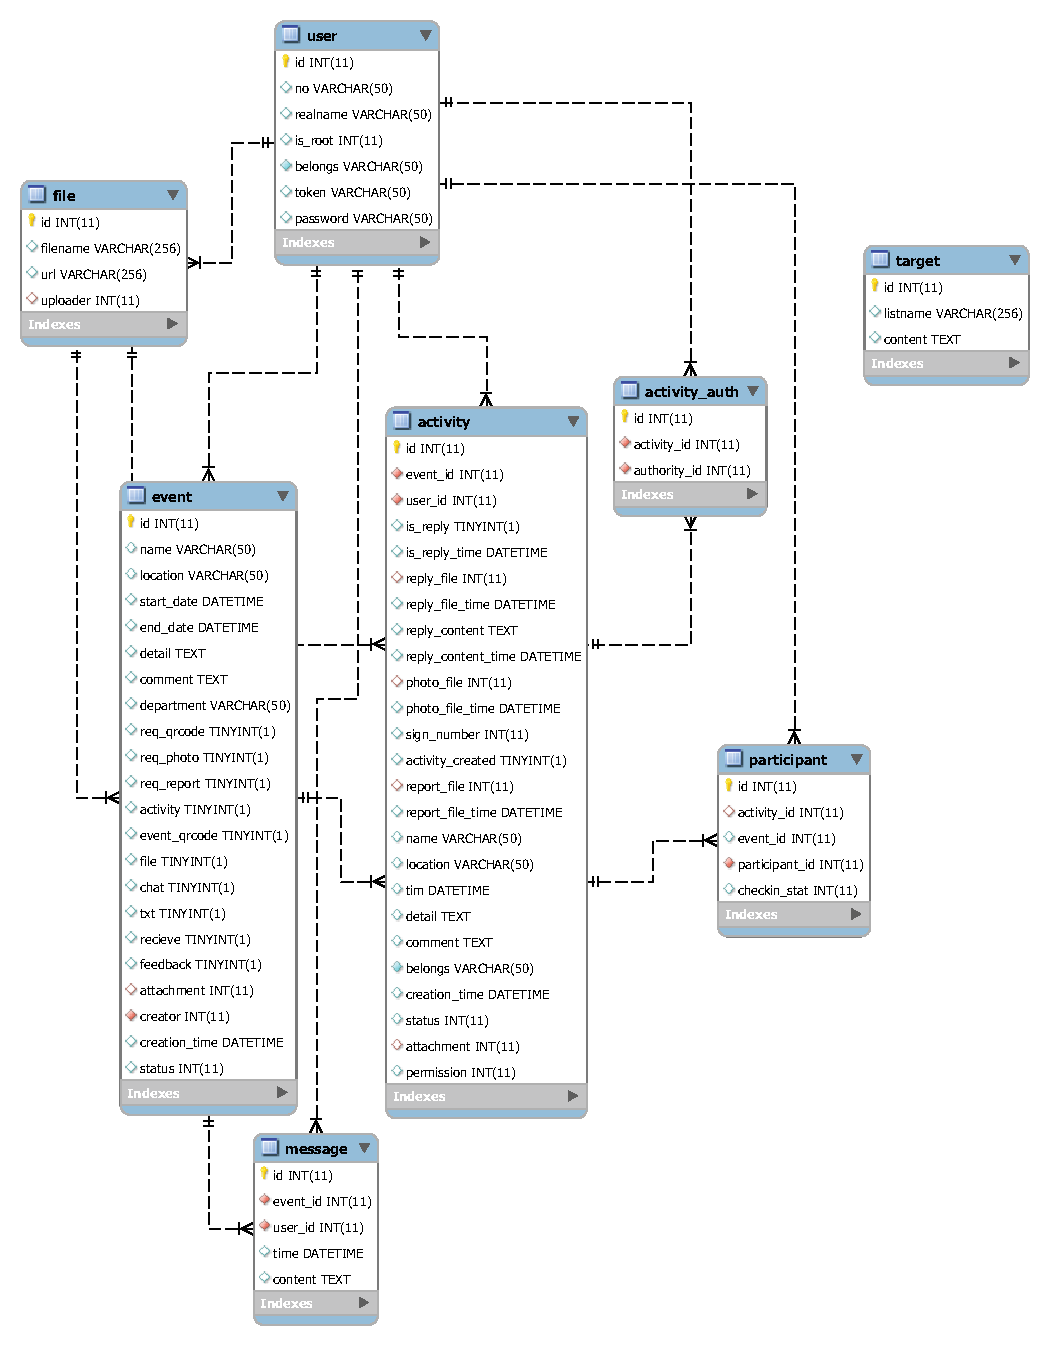
\includegraphics[width=0.8\textwidth]{uml}
  \caption{数据库UML图}
  \label{fig:uml}
\end{figure}

各个数据表的意义如下所述:

\begin{itemize}
\item user:用户数据表,存储了用户相关的信息;
\item file:上传的文件数据表,记录了文件在服务器上的路径、原始文件名以及文件的上传者ID;
\item event:活动数据表,记录了活动的详细信息;
\item activity:子活动数据表,记录了子活动的详细信息;
\item activity\_auth:子活动的授权人,通过两个外链通过一个用户ID和一个活动的ID连接了一个用户和一个活动,表示这个用户是这个活动的授权人之一;
\item message:用户对活动的反馈信息记录表,记录了一个反馈信息所属的活动、用户以及上传时间和反馈内容;
\item participant:记录了一个用户对子活动的参与情况,每一条记录表示了一个用户参与了一个特定的子活动;
\item target: 记录了来自Excel表的发送对象表,通过一个JSON Array保存了一个特定的用户群组。
\end{itemize}

通过对数据库的结构进行设计,可以使得每个API的调用都只会用到一句SQL语句就可以完成所需要的操作,保证了后端运行的效率和反应时间,提高了系统抗压能力,更能够提升用户的体验。

\section{功能详解}

通过\ref{requireAnalysis}节对需求的分析,结合对图\ref{fig:demand2}的分析,我们已经明确了各个角色所需要的功能,接下来需要对系统的具体功能进行设计。

一级管理者拥有对系统最高的控制权,可以指定新的管理员,也可以对分工会主席名单(发送范围)进行修改,并且可以创建只有一级管理者才能创建的活动。对于一级管理者来说,需要使用到的功能如图\ref{fig:level1}所示。

\begin{figure}[H]
  \centering
  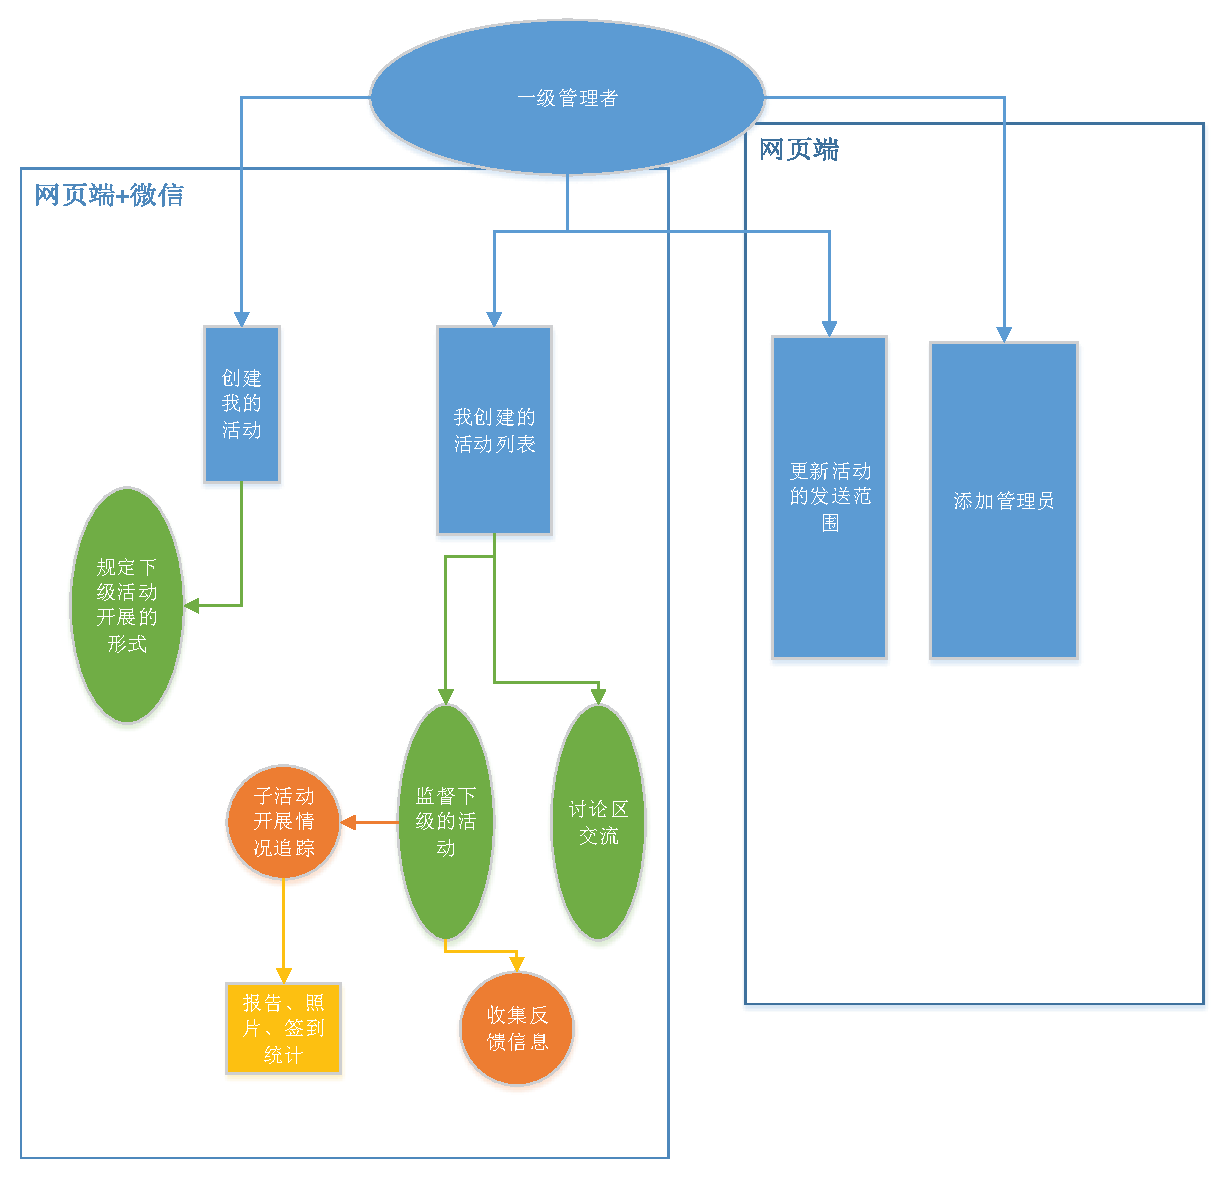
\includegraphics[width=1\textwidth]{level1}
  \caption{一级管理者的功能图}
  \label{fig:level1}
\end{figure}

当一级管理者创建一个活动并将这个活动的消息发送给一些分工会的主席的时候,这些分工会的主席便成为了二级授权者的角色。同时一级管理者可以将自己作为发送范围中的一员,使得自己成为某个活动的二级授权者,从而创建一个活动的子活动。

二级授权者可以将创建子活动的权利授权给另一个用户,使其代自己成为另一个该活动的二级授权者。一个二级授权者可以创建子活动,并对这个子活动进行全权操作。二级授权者的功能图如图\ref{fig:level2}所示。

\begin{figure}[H]
  \centering
  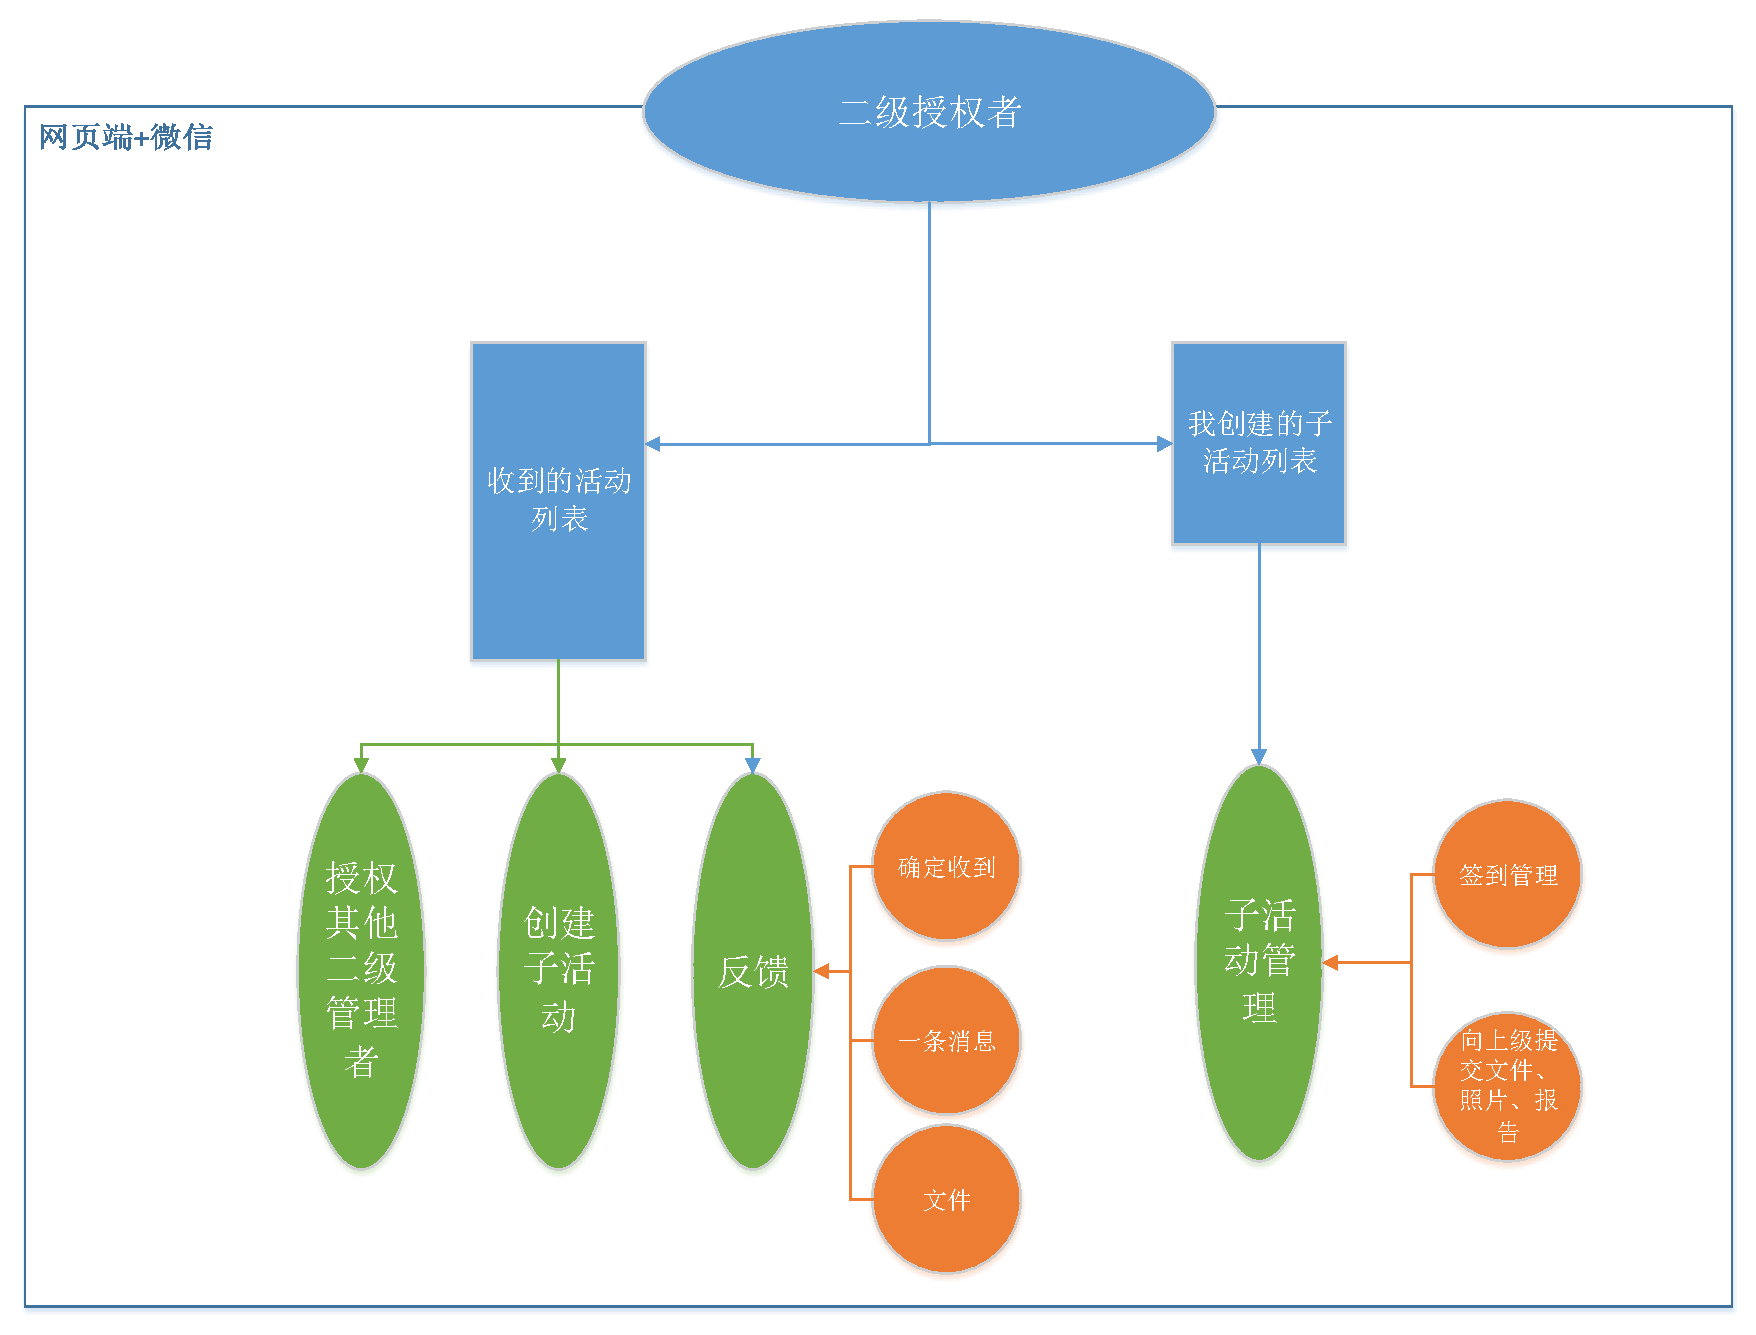
\includegraphics[width=1\textwidth]{level2}
  \caption{二级授权者的功能图}
  \label{fig:level2}
\end{figure}

三级接收者会在二级授权者创建子活动之后,在微信工会公众平台上收到活动信息推送,并选择子活动参与,通过签到确认活动的参与情况。同样的,二级授权者可以参与自己创建的子活动,并成为三级接收者的角色。

三级接收者的权限则十分受限,只能对接收活动和子活动的通知,并通过签到来确认参加活动。三级接收者的功能图如图\ref{fig:level3}所示。

\begin{figure}[H]
  \centering
  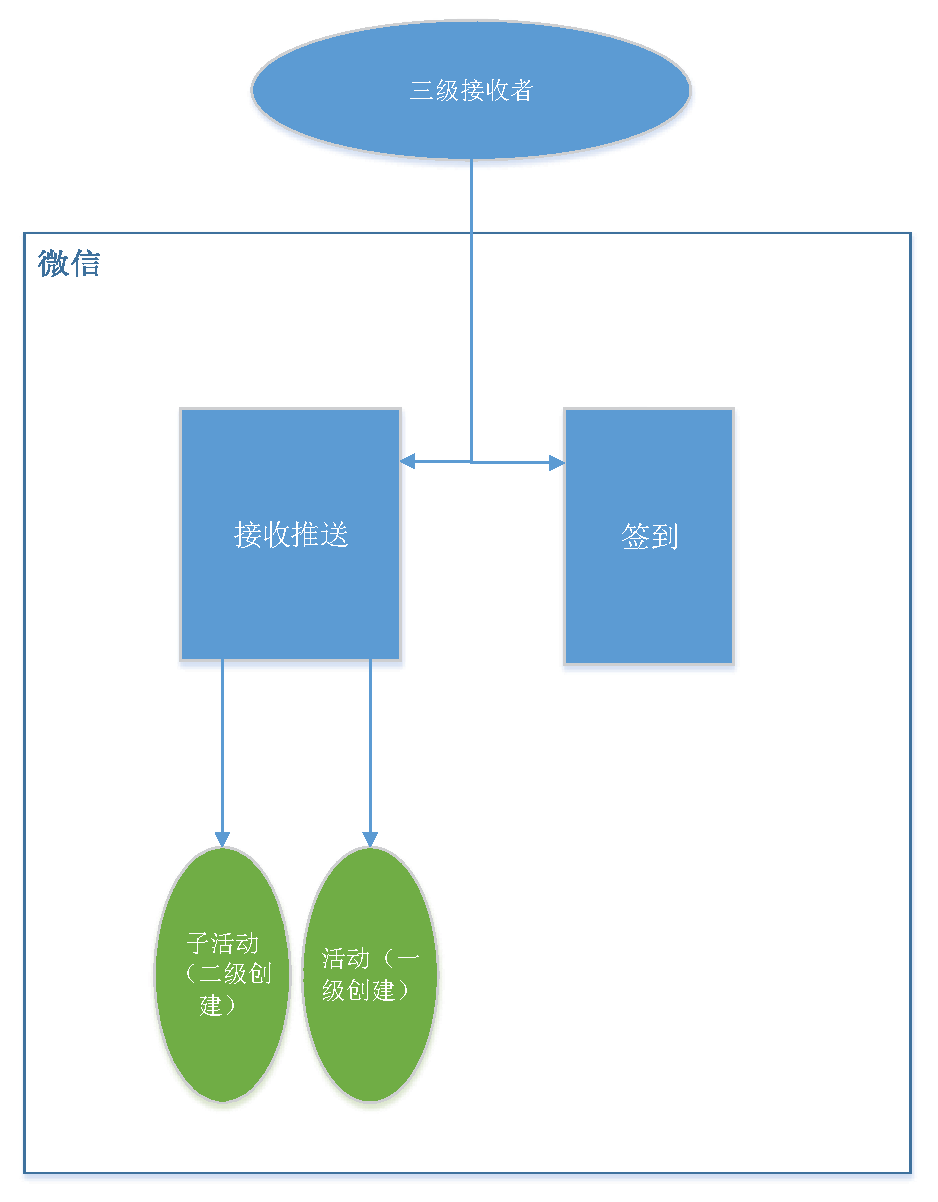
\includegraphics[width=0.6\textwidth]{level3}
  \caption{三级接收者的功能图}
  \label{fig:level3}
\end{figure}

为了完成这些功能,后端需要实现的API如表\ref{table:api}所示。表中给出了系统中用到的全部的API的介绍,以及能够调用该API的用户需要的权限。

\begin{table}[htb]
  \centering
  \caption{后端API表及调用权限}
  \label{table:api}
    \begin{tabular}{llccc}
      \toprule
      API & 描述 & 一级 & 二级 & 三级 \\
      \midrule % $\surd$
      AddActivityAuth 		& 添加一个授权人 			& 	& $\surd$	& \\
      AddParticipant 		& 参与一个子活动 			& 	&  	& $\surd$\\
      CreateActivity 		& 创建一个子活动 			& 	& $\surd$ 	& \\
      EndActivity 			& 结束一个子活动 			& $\surd$	& $\surd$ 	& \\
      GetActivityByEvent 	& 通过活动搜索子活动		& $\surd$	& $\surd$ 	& $\surd$\\
      GetActivityWithEvent 	& 得到一个子活动的详细信息 	& $\surd$	& $\surd$ 	&$\surd$ \\
      GetCreatedActivity 	& 获得当前用户创建的子活动 	& 	& $\surd$ 	& \\
      RenoticeActivity 		& 重新发送活动提醒 			& $\surd$	&  	& \\
      ActivityCheckin 		& 对一个活动进行签到 		& $\surd$	&  	& \\
      GenerateExcel 		& 创建Excel表格报告 		& $\surd$	&  	& \\
      GetCheckedParticipant & 获得一个活动的参与者 		& $\surd$	&  	& \\
      ManualCheckin 		& 手动进行签到 				& 	&  $\surd$	& \\
      CreateEvent 			& 创建一个活动 				& $\surd$	&  	& \\
      GetEventStat 			& 获得一个活动的参与情况 	& $\surd$	&  	& \\
      GetListEvent 			& 获得创建的活动列表 		& $\surd$	&  	& \\
      GetRecvEvent 			& 获得收到的活动列表 		& 	& $\surd$ 	& \\
      GetSingleEvent 		& 获得一个活动的详细信息 	& $\surd$	& $\surd$ 	& \\
      ReplyEvent 			& 对一个活动进行反馈 		& 	&  $\surd$	& \\
      UpdateEvent 			& 更新一个活动内容 			& $\surd$	&  	& \\
      GetFile 				& 得到一个上传的文件详细信息& $\surd$	& $\surd$ 	& $\surd$\\
      UploadFile 		& 上传一个文件 					& $\surd$	& $\surd$ 	& $\surd$\\
      UploadXls 		& 上传一个表格 					& $\surd$	&  	& \\
      GetMessage 		& 得到一个活动的讨论区内容 		& $\surd$	& $\surd$ 	& \\
      NewMessage 		& 添加讨论区内容 				& $\surd$	&  $\surd$	& \\
      UpdateMessage 	& 更新讨论区讨论内容 			& $\surd$	& $\surd$ 	& \\
      DelPostTarget 	& 删除一个用户群组 				& $\surd$	&  	& \\
      GetPostTarget 	& 得到一个用户群组中的用户ID 	& $\surd$	&  	& \\
      NewPostTarget 	& 创建一个新的用户群组 			& $\surd$	&  	& \\
      ChangePassword 	& 修改一个用户的密码 			& $\surd$	& $\surd$ 	&$\surd$ \\
      GetCurrentUser 	& 获得当前用户 					& $\surd$	& $\surd$ 	& $\surd$\\
      GetUserPubKey 	& 为当前登录行为提供一个RSA公钥 & $\surd$	& $\surd$ 	& $\surd$\\
      Login 			& 进行登录行为 					& $\surd$	& $\surd$ 	& $\surd$\\
      Logout 			& 用户登出 						& $\surd$	& $\surd$ 	& $\surd$\\
      SearchUser 		& 查找一个用户 					& $\surd$	&  	& \\
      SetRoot 			& 将一个用户设置为管理员 		& $\surd$	&  	& \\
      SignIn 			& 注册一个新用户 				& $\surd$	& $\surd$ 	&$\surd$ \\
      \bottomrule
    \end{tabular}
\end{table}

实现了这些功能之后,配合前端的界面呈现,系统就能够在各个平台为用户进行服务了。


\chapter{技术要点}

\section{AngularJS}

\label{angularJS}

在HTML5时代之前,一个网页应用通常基于大量的跳转链接,以及凌乱的布局和滚动条来完成相应的操作。和“网页应用”这个概念不同的是,传统的网页服务往往是“链接驱动”的。随着互联网技术的发展,提供服务的网页也越来越像一个独立的应用。而AngularJS的横空出世,更是为传统网页设计模式画下了终止符。

AngularJS是一款优秀的前端Javascirpt框架,具有强大的模板功能,使用Angular声明式的指令代替传统的HTML和Javascript的指令,使得AngularJS具有了强大的数据绑定能力。通过AngularJS的双向数据绑定功能,应用逻辑可以从DOM操作中解耦出来,使得开发者能够专注于逻辑的开发而不用为数据的呈现伤脑筋。

此外,AngularJS是一个完善的MVC框架,提供了模板、路由、模块化、过滤器、依赖注入等一系列原先需要用一个单独的后端才能实现的功能,避免在本文的系统中出现两套后端的情况,极大地简化了开发。其中AngularJS提供的Angular-router路由功能能够对网页的URL进行解析,使得页面在不被刷新的情况下,更新在页面上显示的内容。

使用AngularJS的模板和directive功能,可以使得原先静态的元素或者只能在后端进行拼装的前端网页元素能够被方便地复用,十分适合用于应用的UI开发。例如在本系统中,使用directive功能开发的文件上传组件被插装在了系统的各个位置,避免了对文件上传按钮的重复开发,同时也使得界面统一,提升了用户体验。

在AngularJS的基础上,有许多优秀的扩展,其中在本系统中用到的还有Angular Mobile和Angular Mateiral。

Angular Mobile是一个基于Angular和Bootstrap的UI前端开发框架,专门用于在手机浏览器上的网页提供类似移动设备原生应用类似的用户体验,方便开发者开发HTML5移动应用。因此Angular Mobile十分贴合清华大学工会系统的需求。因此微信端的管理平台就是基于Angular Mobile开发设计的。其丰富的网页元素控件不仅节省了我们大量的开发时间成本,而且还为用户提供了一个干净整洁的界面。

另一方面,在系统的浏览器端则使用了Angular Material作为UI框架。这是由于浏览器端相对手机浏览器拥有更强的处理和计算能力。搭配Angular Material的大量UI素材以及活泼的网页动画,使用Angular Material使得系统的前端更加生动而易于使用。

\section{REST架构}

\label{rest}

传统的基于Servlet的网页应用通常离不开对JSP的依赖。使用JSP来呈现网页内容,并在JSP中嵌入后端的JAVA代码不失是一种简单的开发模式。然而当一个网页应用存在多个不同版本的前端的时候,使用JSP和Servlet的模式就受到了挑战:必须对每个前端的版本都配备一套JSP代码,每次前端修改的时候,都必须重新载入后端。这不仅令服务器的热更新不可行,更在前端需要被部署在远程的时候受到了更严重的挑战:JSP无法被部署在远程服务器上,它与Servlet的耦合太紧了。

一个解决方法就是使用REST架构。这是一个使用JSON和AJAX技术作为前后端沟通的技术。前端通过带有参数的AJAX请求,对后端的Servlet发出HTTP请求,并获得来自后端的反馈结果。

通过这样设计的前后端通讯方法可以使得后端不需要考虑前端是如何实现的,而仅仅需要对JSON的参数格式做出约定就可以完成前端对后端功能的调用工作。使用这种方法可以使得同一套后端的服务器可以同时为多套前端应用提供服务,而不用对后端的服务例程进行重写。

应用在本文的系统中,微信前端和网页端的前端的实现方式存在较大的差异,两者有着截然不同的controller控制器。在这种情况下,后端依然能够同时为两个前端提供服务,就是凭借了REST架构中将AJAX和JSON作为沟通前后端的方式提供的灵活性来完成的。

\section{基于会话的身份认证}

对于网页应用来说,前端的操作不是永远都是安全的。换句话说,后端需要保证发送给前端的数据不会导致危险的事情发生。比如,一旦将当前用户的身份认证工作交给前端来做,那么不怀好意的前端用户就可以通过修改前端的身份认证流程,使得自己能够以别人的身份进行操作,并对系统产生不可预计的破坏。因此,后端需要有一个合适的方法来对当前登录的用户信息进行管理。

但是麻烦的是,HTTP是无状态网络连接,也就意味着每次新请求都不会记得上一次请求的任何来自后端的信息,而前端的Cookie又是不可信的。这使得如何记录下当前已经登录的用户身份成为一个棘手的问题。

\subsection{浏览器端的身份记录}

对于基于Servlet架构的后端来说,一个可行的方案是使用会话(session)机制。

理想的Session是一个当用户在应用程序的Web页之间进行跳转的时候,Session记录不会丢失。对于JAVA Servlet来说,Session就是一个特殊的不可复制的Cookie。

如何令一个Cookie不可被伪造?即当会话建立用户登录的时候,Servlet会向用户发送一个SetCookie请求,其中包含了一个名为JSESSIONID的Cookie。这个Cookie是一个后端随机生成的16进制大数字。每次进行API调用的时候,浏览器都会自动将JSESSIONID这个Cookie随着HTTP请求一道发向后端服务器。后端服务器会尝试获得拥有这个Session ID的用户信息作为该终端中登录的用户。除非一个心怀鬼胎的用户能够以极低的概率蒙对另一个人的Session ID,否则他将无法通过修改Cookie的方法将自己终端上已经登录的用户修改成他人。

在本系统中,对session的使用如图\ref{fig:sessionIn}和图\ref{fig:sessionOut}所示。

\begin{figure}[H]
  \centering
  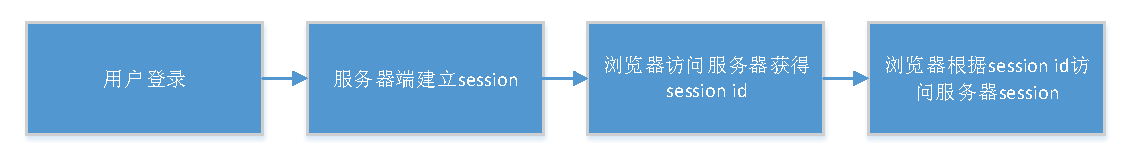
\includegraphics[width=1\textwidth]{sessionIn}
  \caption{创建Session的过程}
  \label{fig:sessionIn}
\end{figure}

\begin{figure}[H]
  \centering
  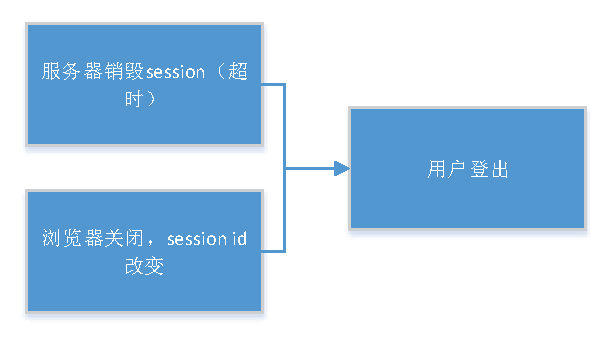
\includegraphics[width=0.5\textwidth]{sessionOut}
  \caption{销毁Session的过程}
  \label{fig:sessionOut}
\end{figure}

通过这样的控制,当前登录的用户就能够被很好地记录下来了。

\subsection{微信中的身份记录}

在微信中,同样需要对用户当前的身份进行识别工作。对于微信的使用者来说,在移动设备上输入用户名和密码是一件十分痛苦的事情。参考清华大学企业号的实现,系统中微信部分的身份识别工作通过ticket的方式来进行。在微信客户端中的每一次操作都会生成一个与用户唯一对应的ticket信息。类似JSESSIONID,ticket同样是一串不可被复制的可以信任的身份凭证。通过对微信服务器的查询,可以得到拥有这个ticket的用户信息,并通过用户信息反向查询得到用户的工作证号,如图\ref{fig:wechatAuth}的流程所表述的那样。

\begin{figure}[H]
  \centering
  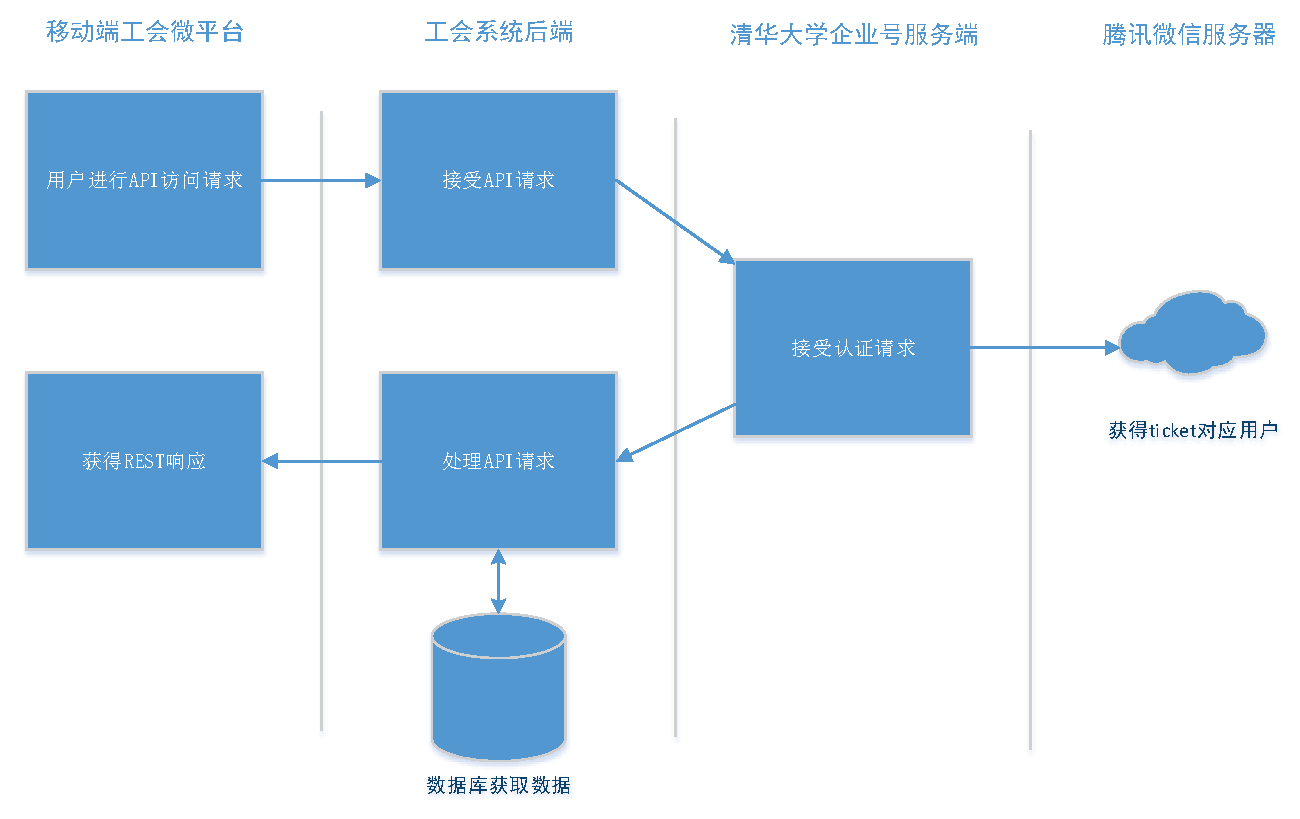
\includegraphics[width=1\textwidth]{wechatAuth}
  \caption{清华大学工会微信微平台用户认证流程}
  \label{fig:wechatAuth}
\end{figure}

通过ticket方式获得工作证号的方法避免了用户在移动设备上进行输入的繁琐,只需要其登录了微信客户端就可以通过微信认证的方式免登录地操作清华大学的工会系统了。同时这种方式也保证了用户信息的安全性,将其他的安全风险分摊到腾讯的微信服务当中去。

\section{RSA加密}

由于HTTP协议的不安全性,如果将用户名和密码等存在隐私问题的数据直接通过HTTP协议传输,那么一旦被截获就会产生密码泄露的安全问题。虽然HTTPS协议可以解决这一安全问题,但是HTTPS并不是每个服务器都可以申请进行的,绝大多数网站依然运行在HTTP协议上。

不可避免的,清华大学工会管理系统也遇到了同样的问题。系统在需要用户进行登录。在网页端进行登录的时候用户的身份验证使用的是密码。如果对密码进行可逆的加密传输,就会导致密码容易被截获并导致个人信息泄露。如果泄露的是管理员的密码信息,还会导致更严重的后果。

系统中用到的RSA认证过程如图\ref{fig:rsa}所示。

\begin{figure}[H]
  \centering
  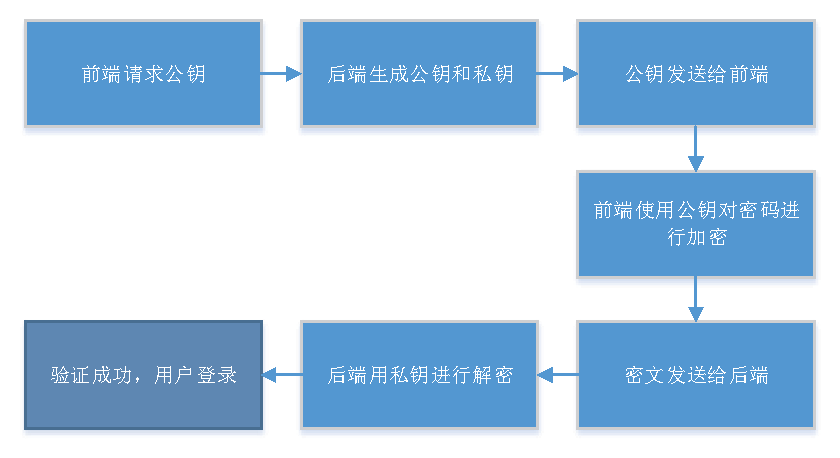
\includegraphics[width=0.8\textwidth]{rsa}
  \caption{销毁Session的过程}
  \label{fig:rsa}
\end{figure}

为了保护使用系统的用户的信息安全,在用户进行登录行为的时候,系统后端会使用OpenSSL工具根据用户名生成一对RSA公钥私钥对,并将公钥发送到前端。前端使用jsencypt.js对密码用公钥加密,并将加密后的密码连同用户名发给后端请求验证。后端将使用RSA私钥对加密后的密码进行解密,如果解密后的结果和数据库中的密码一致,则认为登录成功,创建会话并返回结果;否则登录行为将被拒绝。

通过这种方式,用户的密码能够获得很好的保护,防止由于网络窃听而导致的密码泄露问题。


\chapter{成果与对比}

\section{成果展示}

本文着重对系统的架构进行了介绍,同时也实现了一个功能完整,包含全部文章中所提到技术和功能点,以及符合文中陈述的开发框架的清华大学工会管理系统,以此来证明文中所述的系统架构能够投入到实际运用,是行之有效的工程系统框架。

\subsection{B/S浏览器端}

接下来将通过一系列的图片和描述来模拟开展一个公会活动的过程。

首先,总工会主席需要通过上传一份公会人员名单来创建一个群组。图\ref{fig:postTarget}展示了工会主席创建工会人员群组的过程。

\begin{figure}[H]
  \centering
  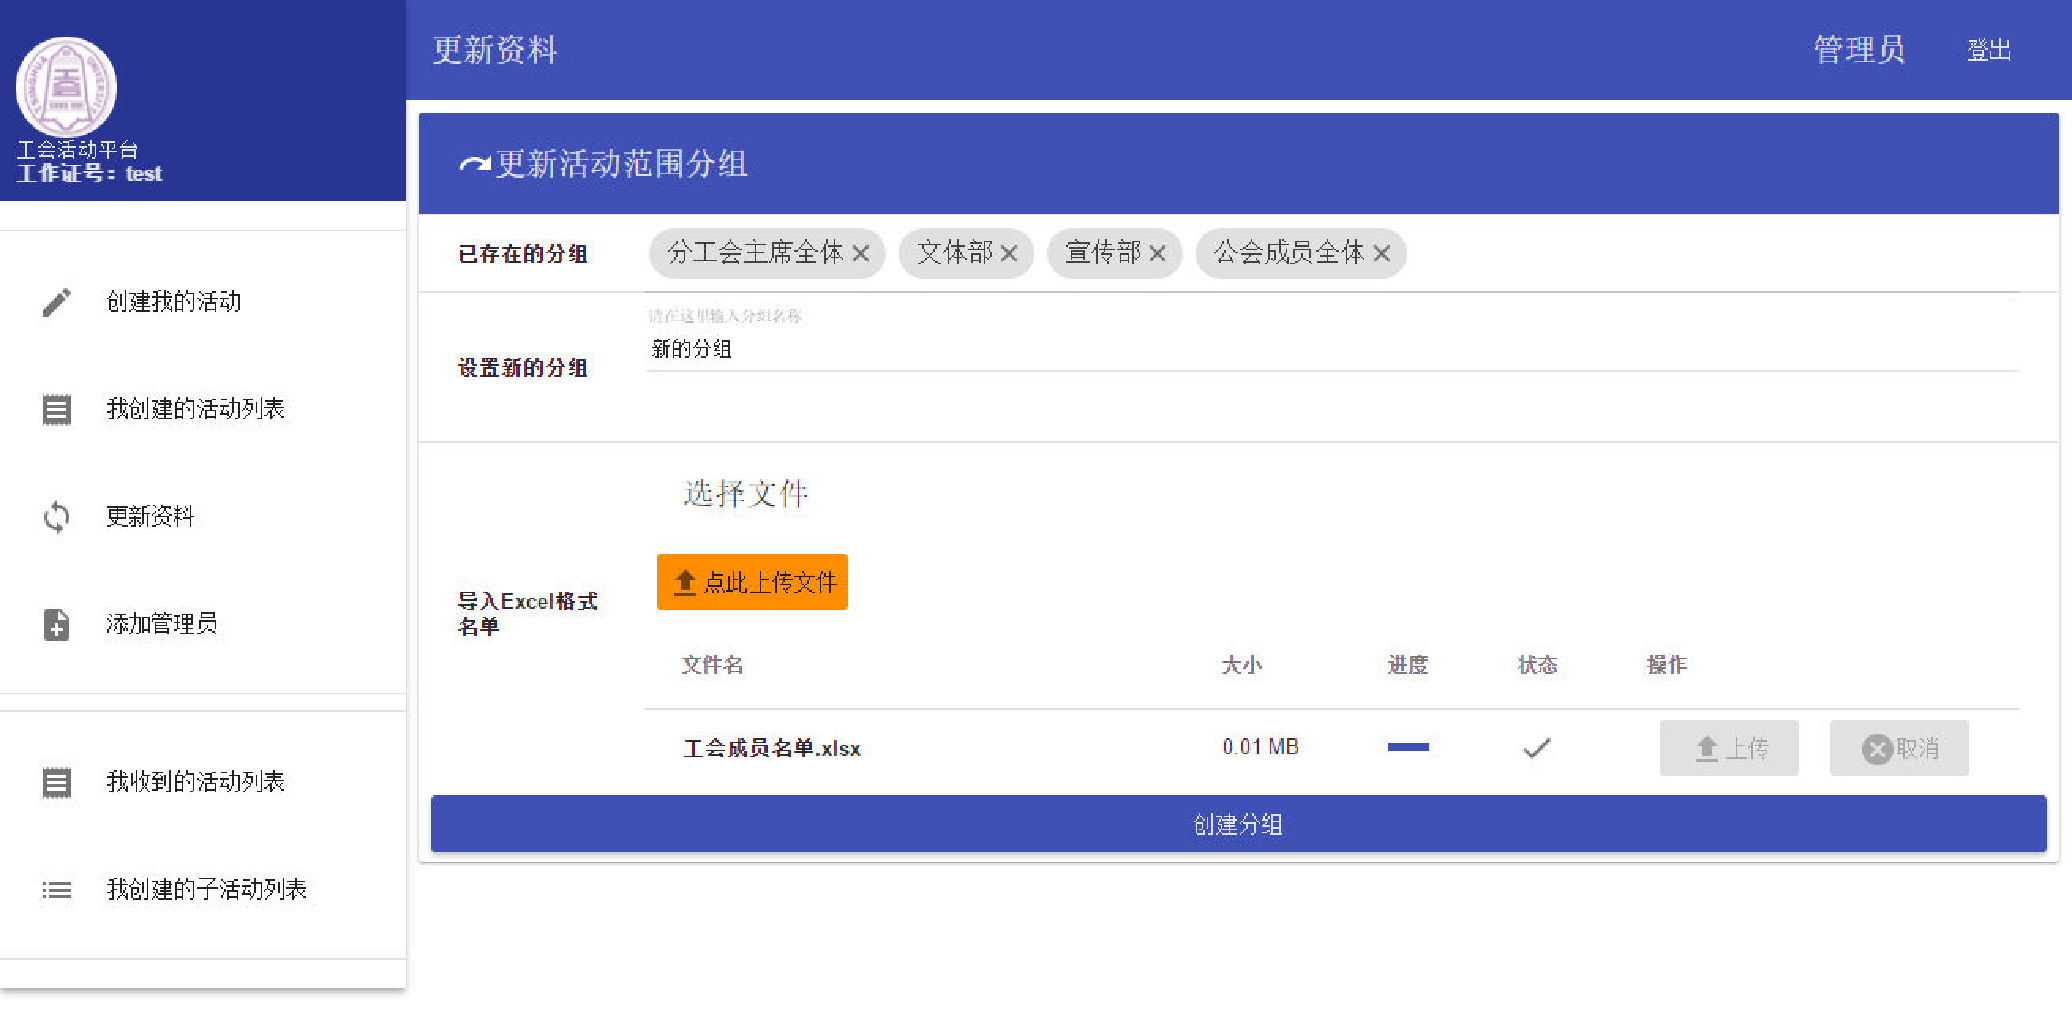
\includegraphics[width=0.8\textwidth]{postTarget.pdf}
  \caption{总工会主席创建群组}
  \label{fig:postTarget}
\end{figure}

在完成了群组创建过程之后,工会主席就可以创建一个新的活动并且指定刚刚创建的群组作为活动通知下达的对象进行发送。图\ref{fig:createEvent}展示了工会主席创建活动时的界面。

\begin{figure}[H]
  \centering
  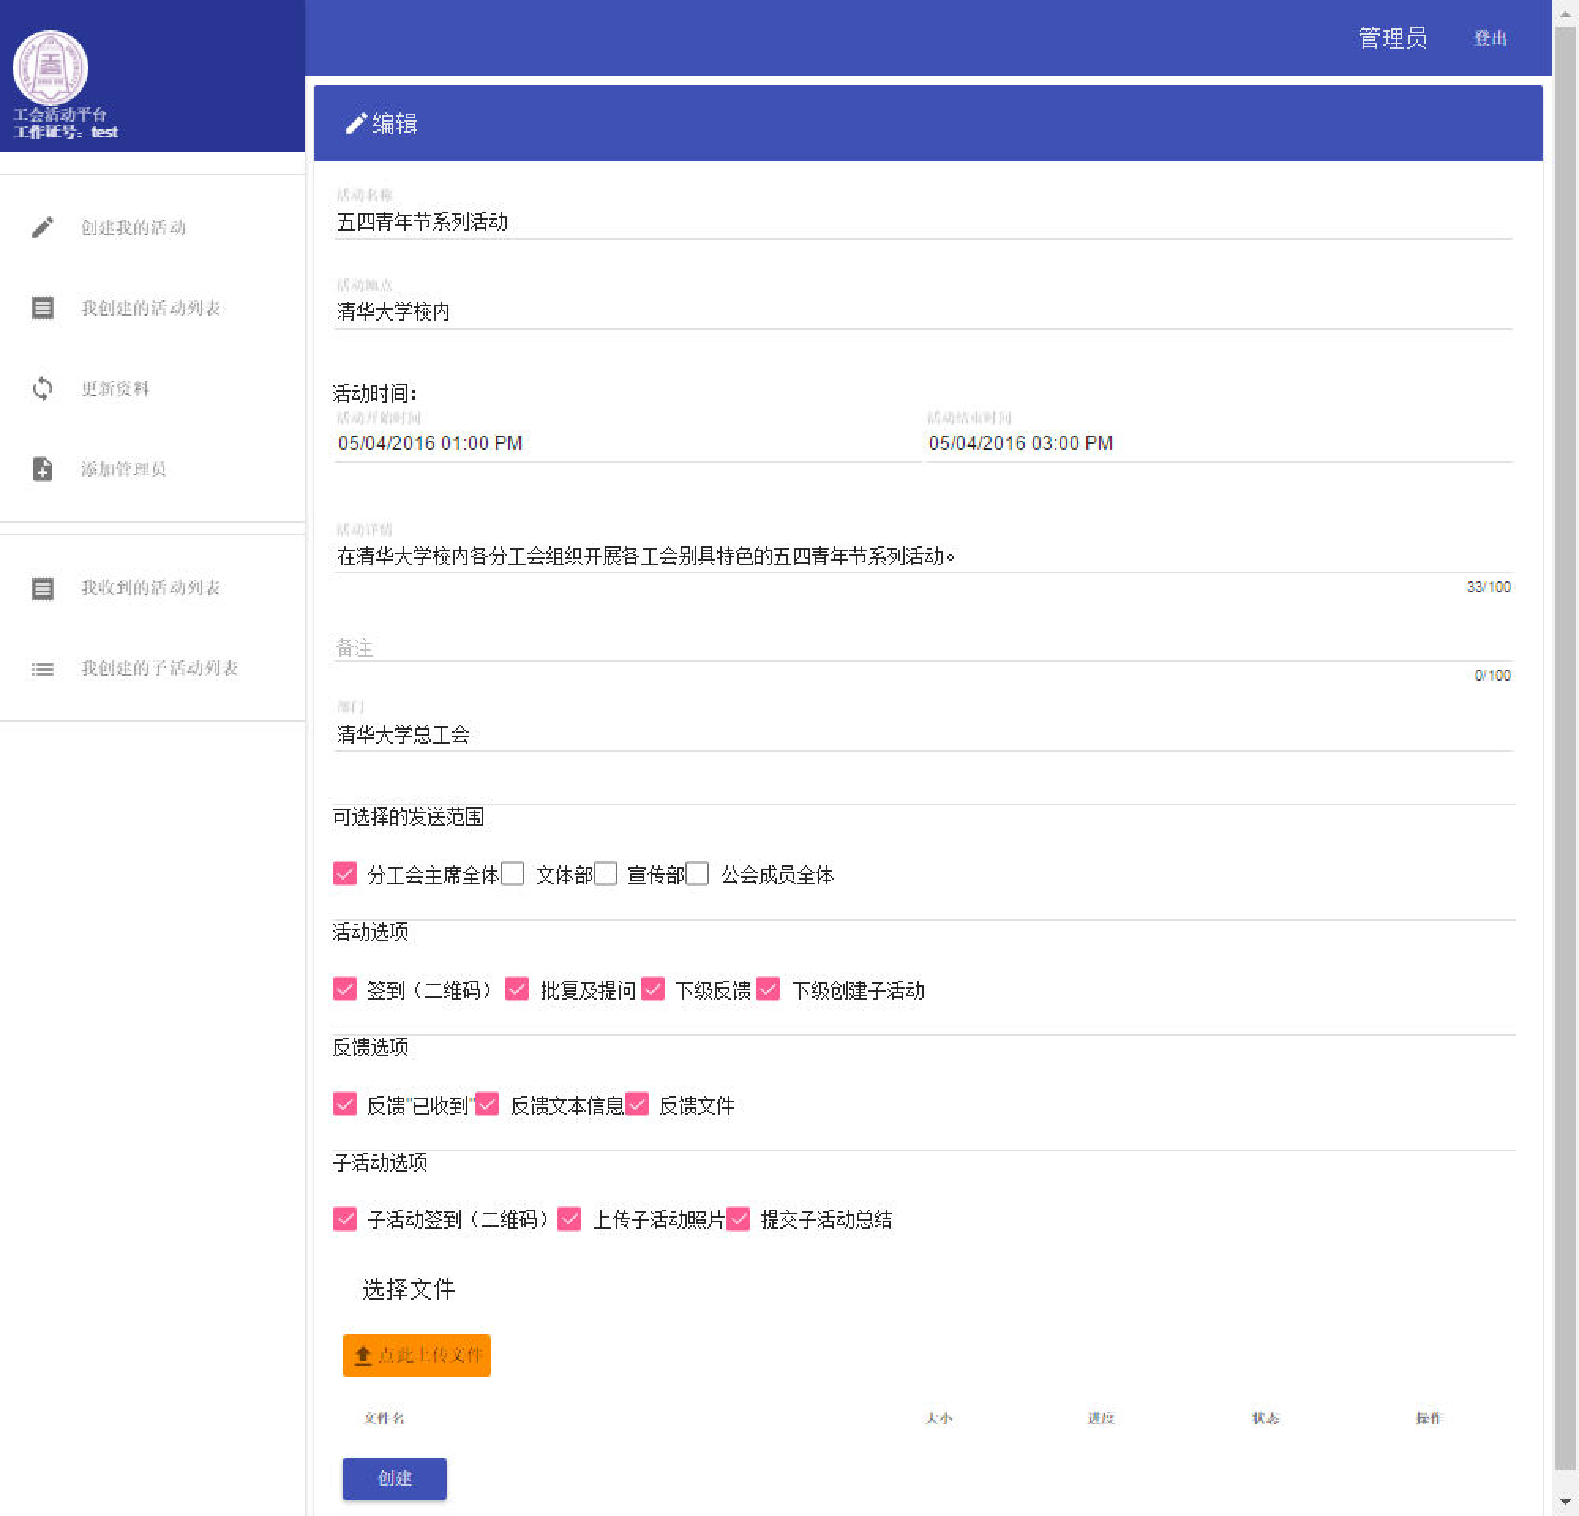
\includegraphics[width=0.8\textwidth]{createEvent.pdf}
  \caption{总工会主席创建一个新的活动}
  \label{fig:createEvent}
\end{figure}

完成活动创建之后,工会主席就能够在图\ref{fig:eventList}中查看到自己创建的活动列表了。

\begin{figure}[H]
  \centering
  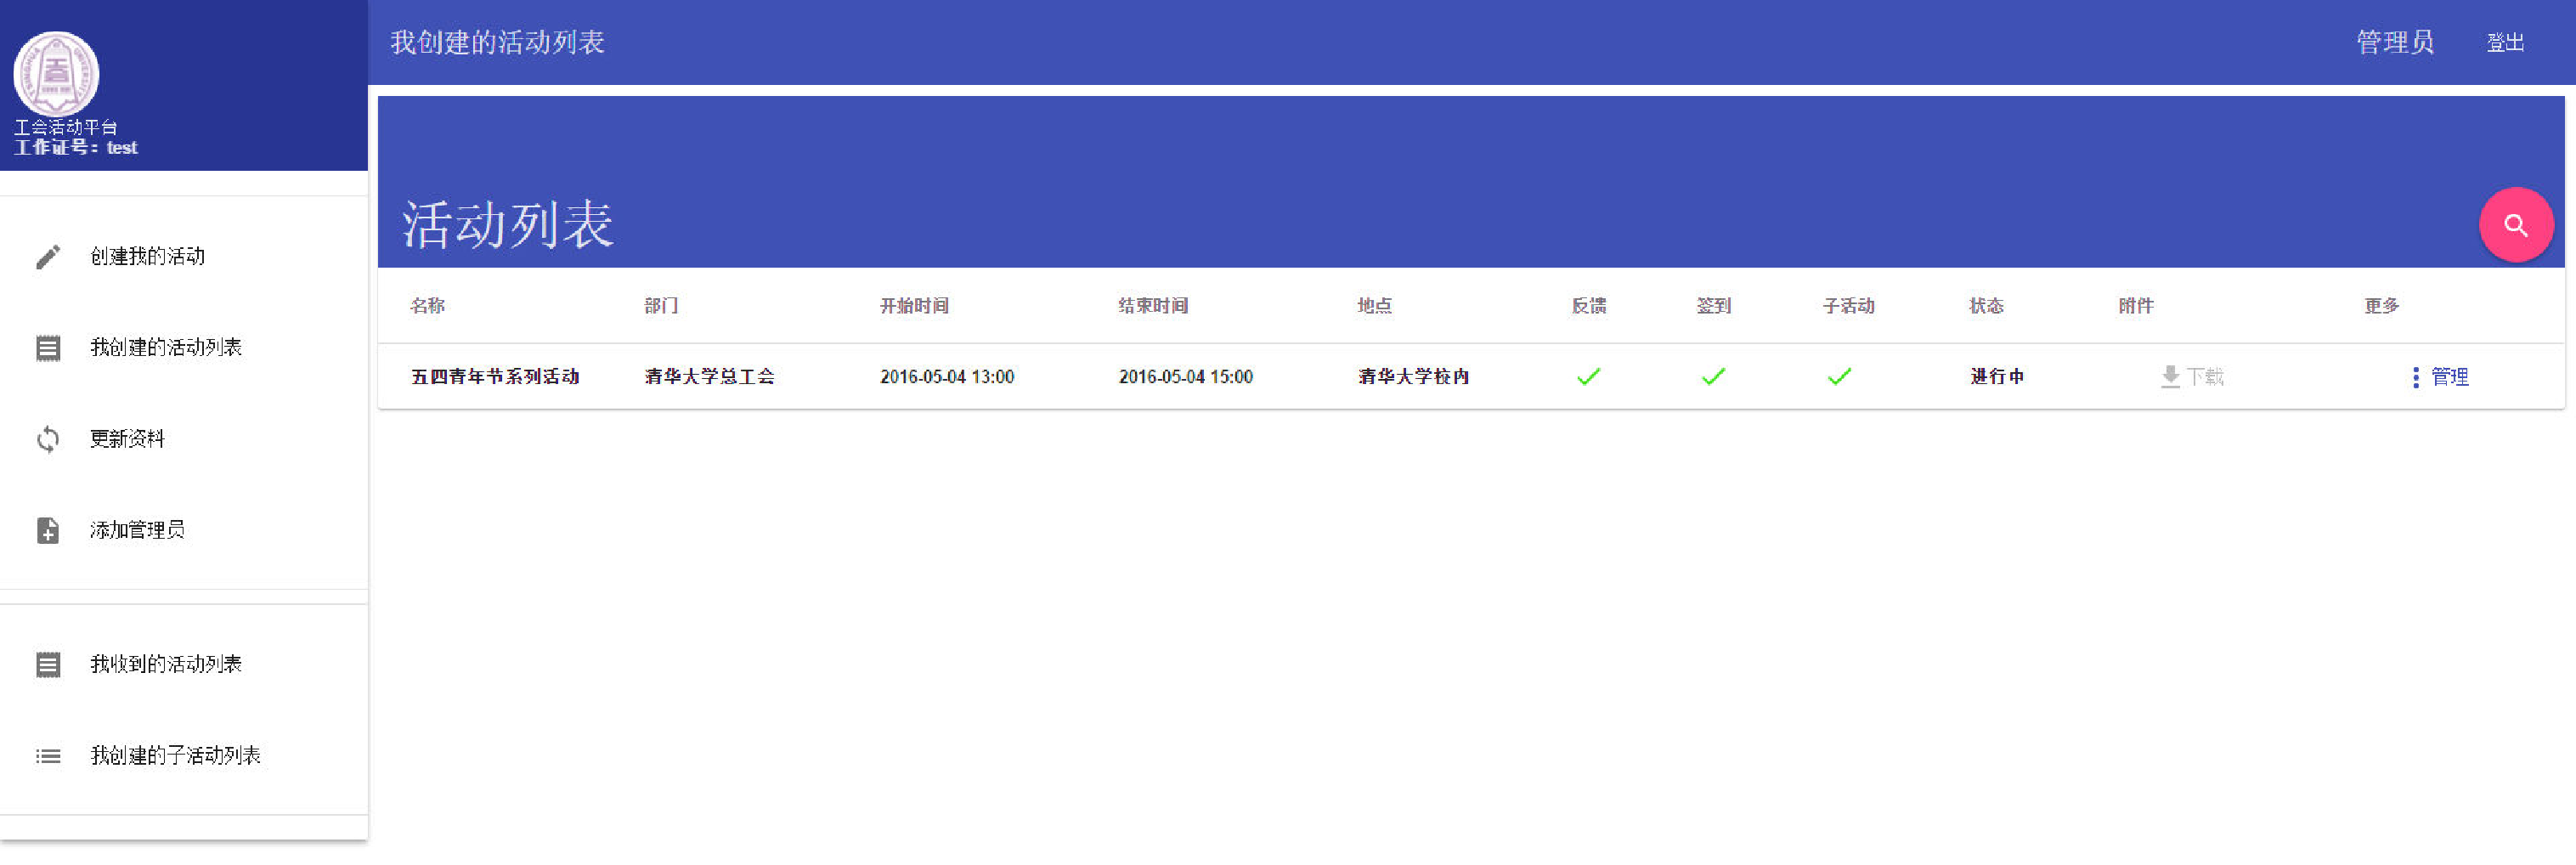
\includegraphics[width=0.8\textwidth]{eventList.pdf}
  \caption{总工会主席创建的活动列表}
  \label{fig:eventList}
\end{figure}

此时收到这个活动的分工会主席就可以登录到系统中并查看到自己已经收到了这个活动的通知(图\ref{fig:activityList})。在图\ref{fig:activityDetail}所示收到的活动详情页中,分工会主席可以针对活动的需求来完成相应的工作。

\begin{figure}[H]
  \centering
  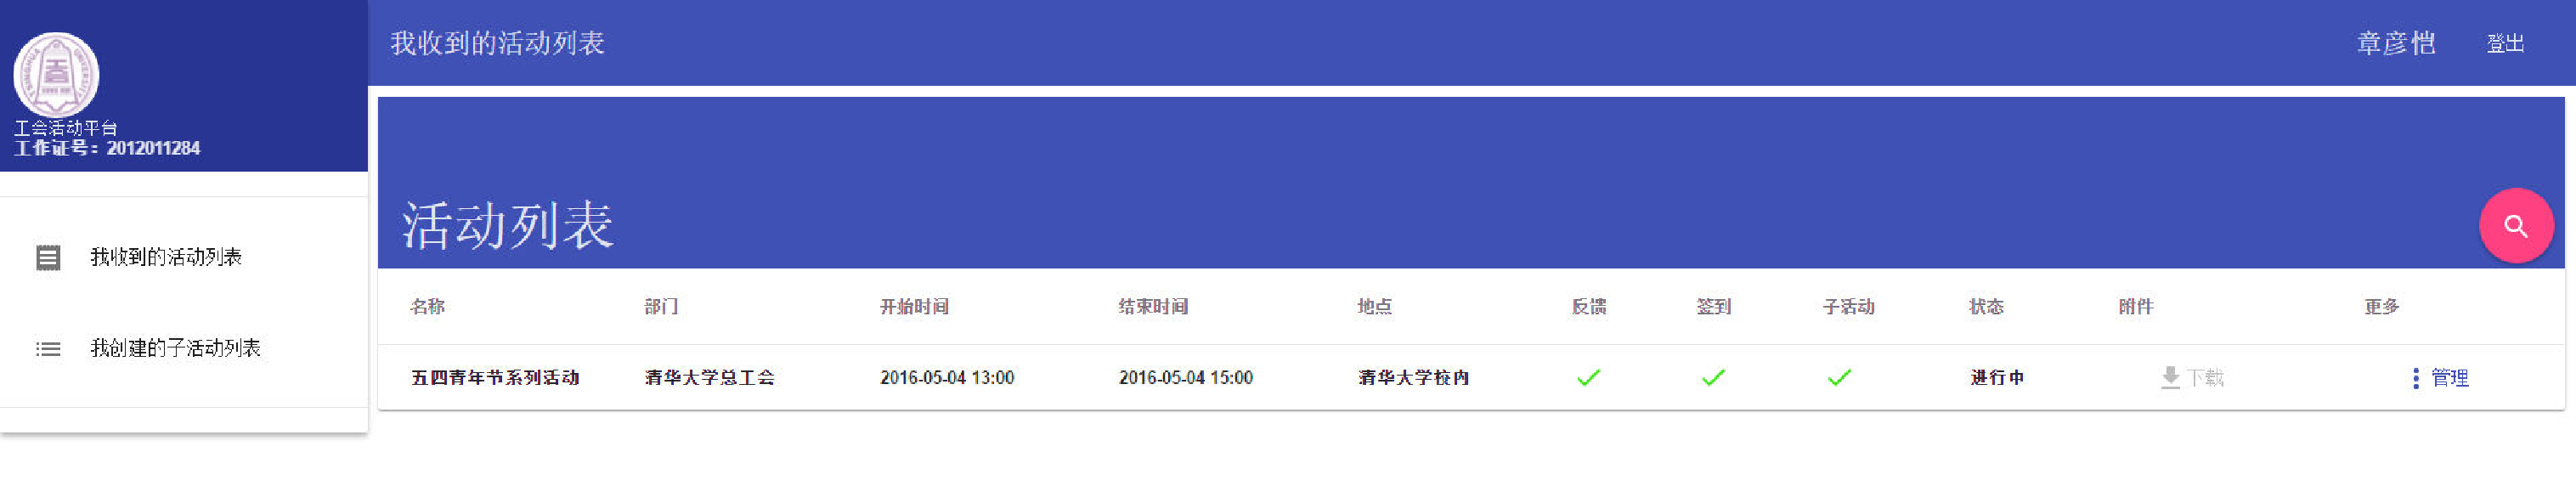
\includegraphics[width=0.8\textwidth]{activityList.pdf}
  \caption{分工会主席收到的活动列表显示}
  \label{fig:activityList}
\end{figure}

\begin{figure}[H]
  \centering
  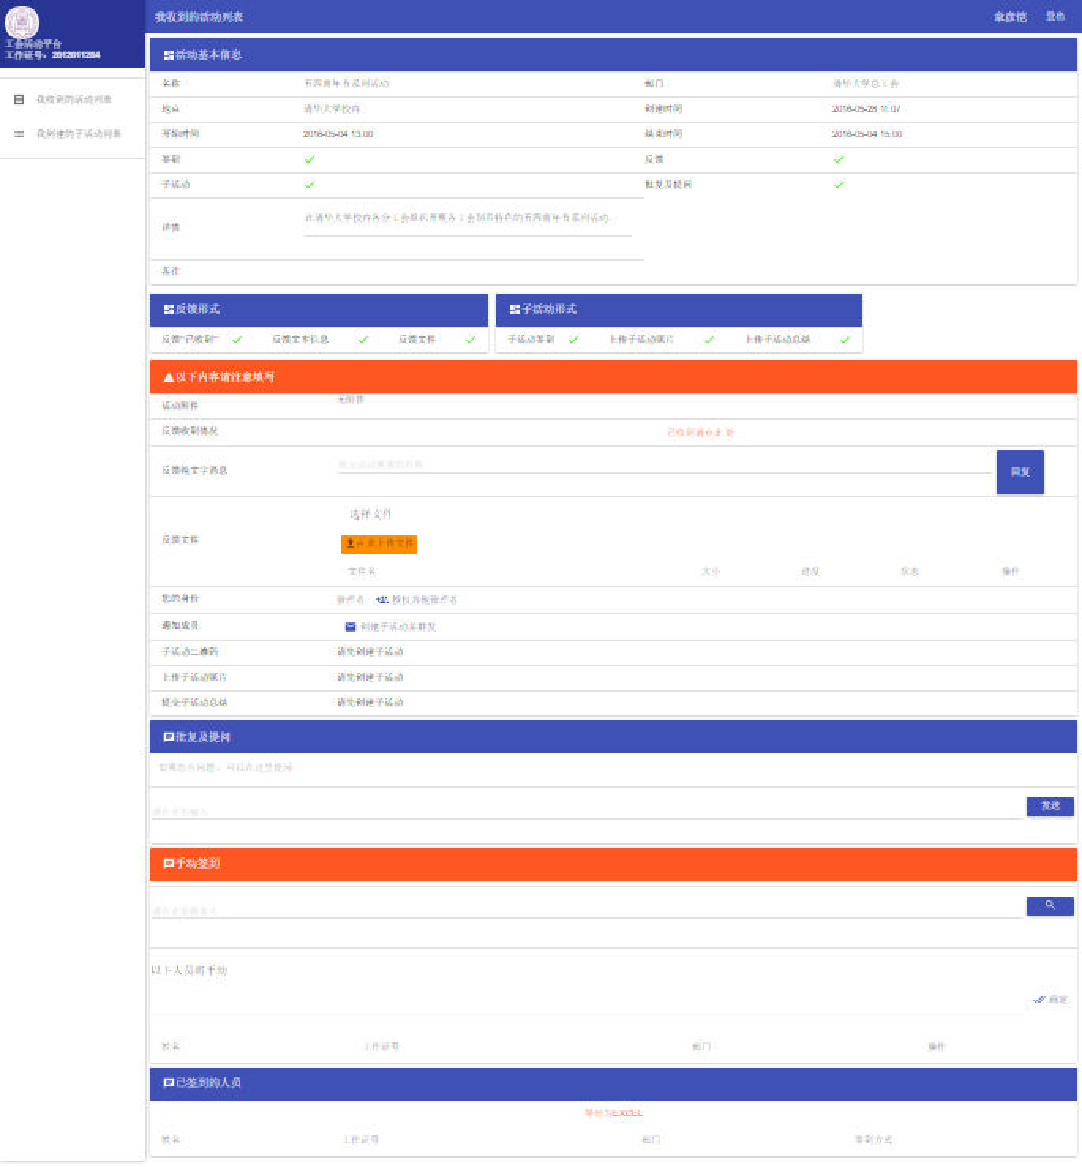
\includegraphics[width=0.8\textwidth]{activityDetail.pdf}
  \caption{分工会主席收到的活动详情页面}
  \label{fig:activityDetail}
\end{figure}

由于创建的活动需要分工会主席开展子活动,因此分工会主席需要点击“开展子活动”按钮,并填写子活动的详细信息(图\ref{fig:shotActivity})。

\begin{figure}[H]
  \centering
  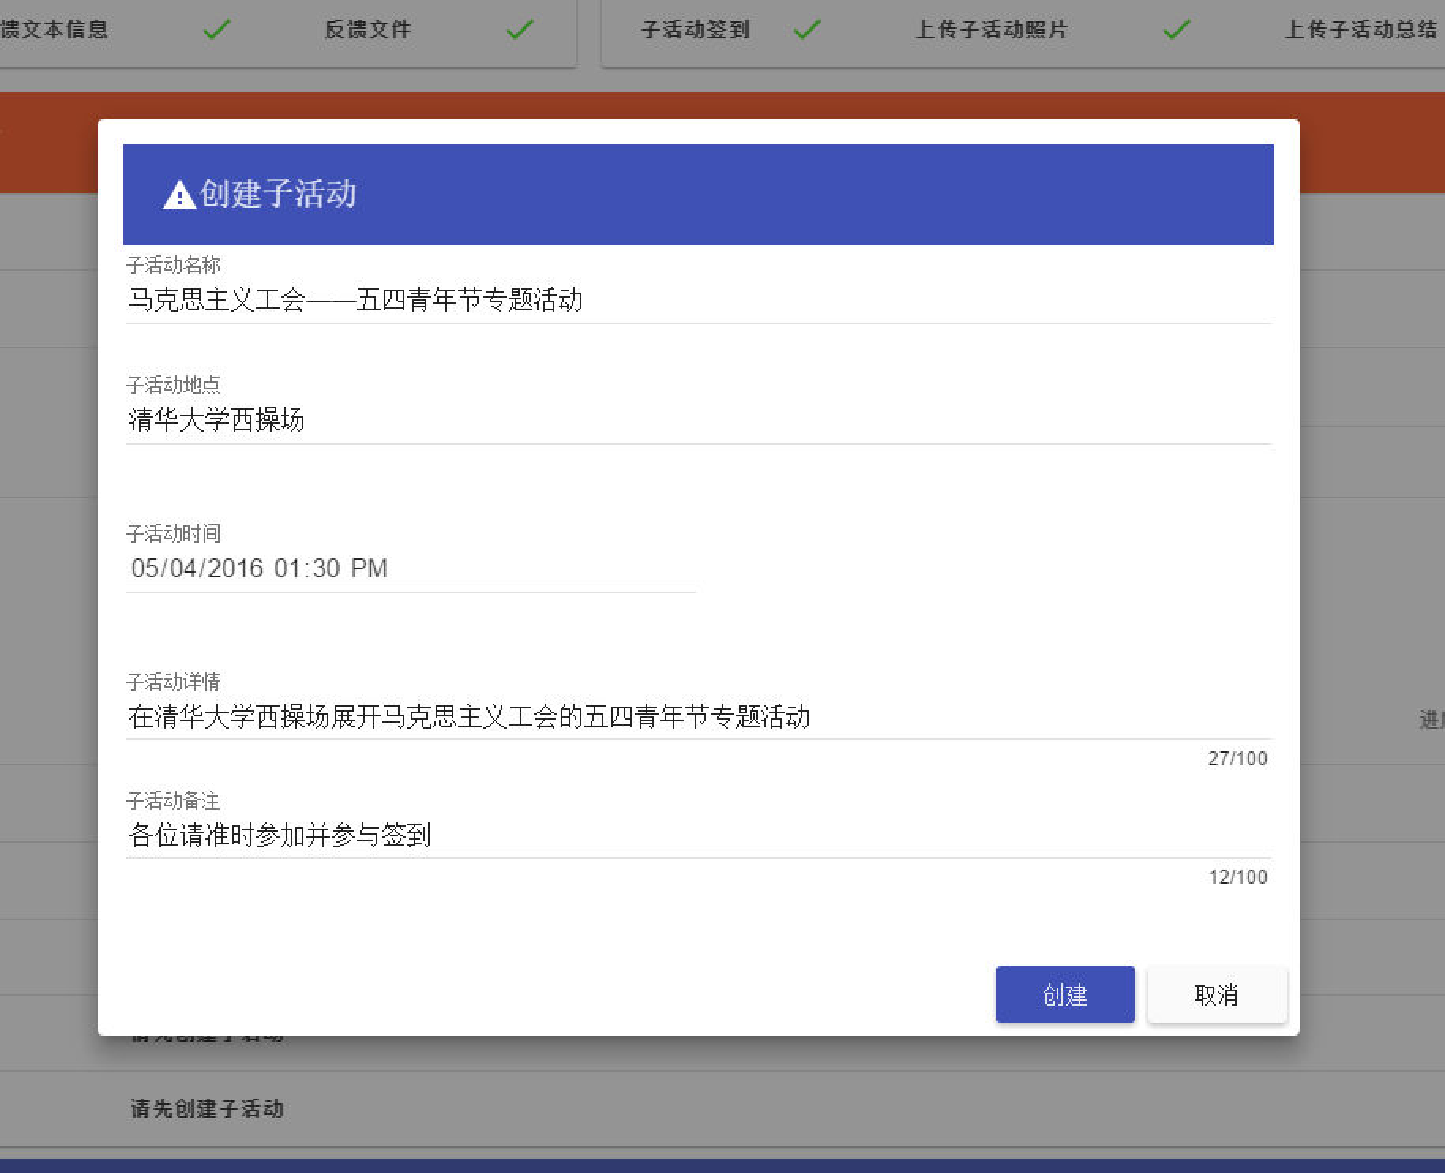
\includegraphics[width=0.8\textwidth]{shotActivity.pdf}
  \caption{分工会主席填写子活动详细信息并创建子活动}
  \label{fig:shotActivity}
\end{figure}

在完成子活动创建之后,工会成员就会收到新的可以参加的活动通知了,如图\ref{fig:shotPost}。

同时,分工会主席在详情页中可以就活动的需求向工会主席提出问题,工会主席可以对这些问题进行回答,如图\ref{fig:message}所示。

\begin{figure}[H]
  \centering
  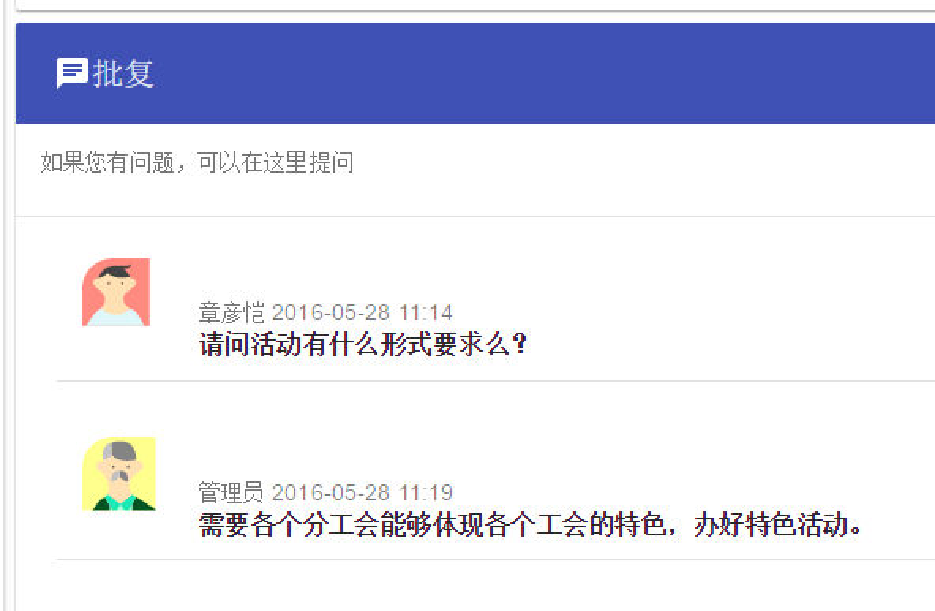
\includegraphics[width=0.8\textwidth]{message.pdf}
  \caption{分工会主席与工会主席通过系统进行提问和回答}
  \label{fig:message}
\end{figure}

当子活动的状态发生变化的时候,总工会主席可以在活动的详情页中看到该活动所有下属子活动以及活动本身的统计信息记录。图\ref{fig:eventDetail}即为“五四青年节系列活动”的详情页展示。

\begin{figure}[H]
  \centering
  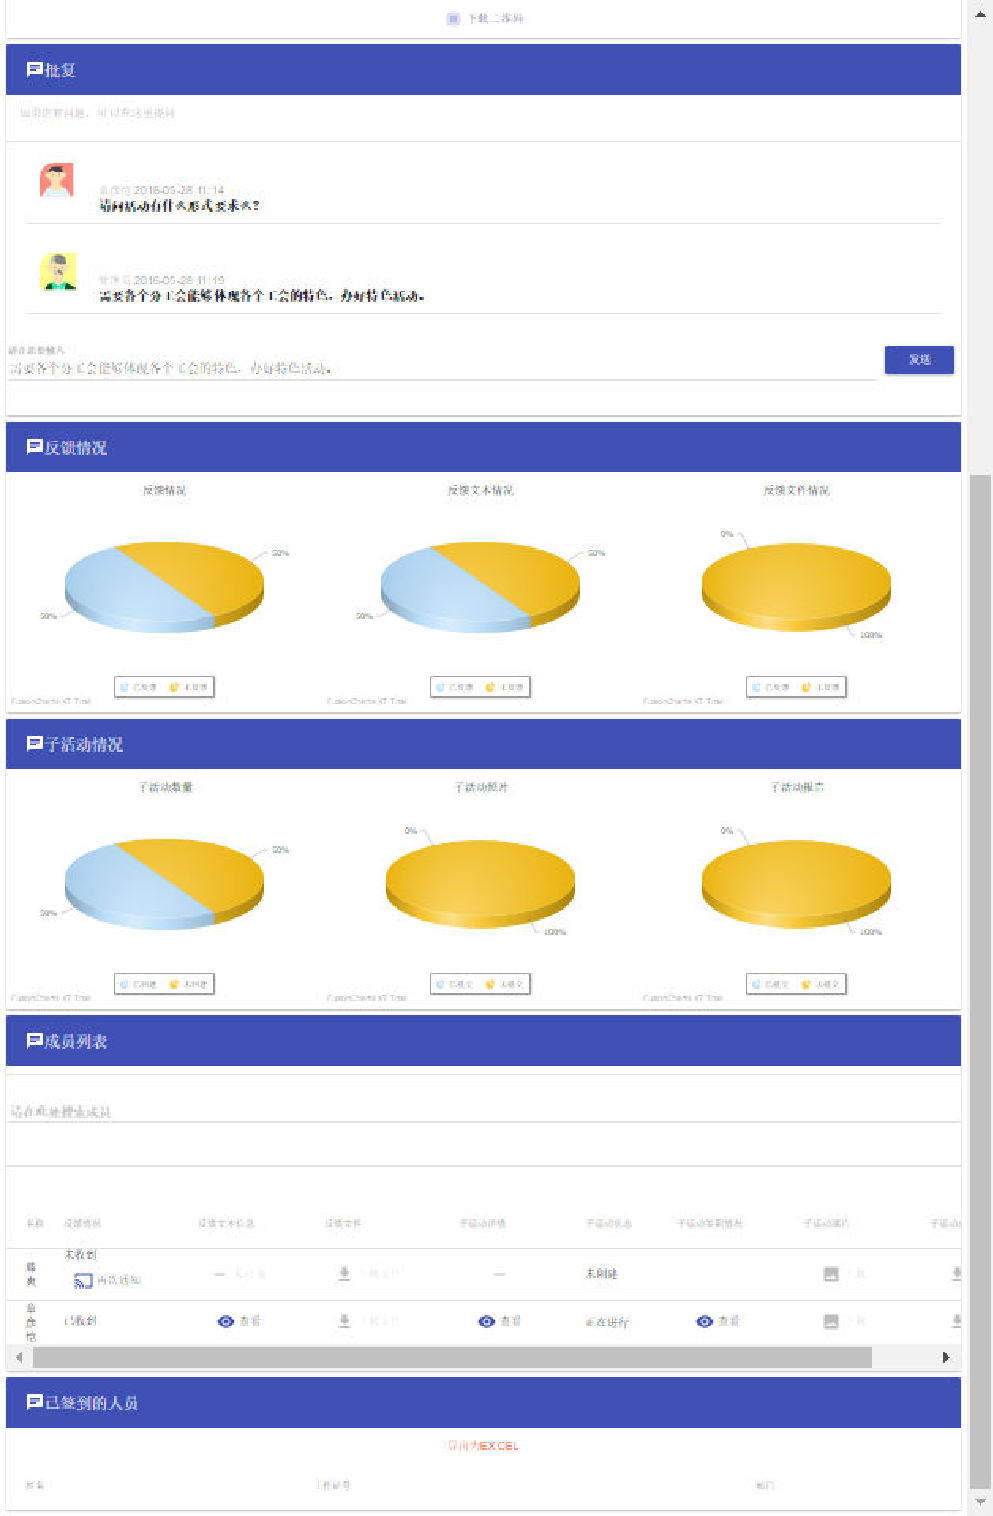
\includegraphics[width=0.8\textwidth]{eventDetail.pdf}
  \caption{工会主席在活动的详情页中看到的活动开展情况统计}
  \label{fig:eventDetail}
\end{figure}

在网页客户端中可以对一个活动进行手动签到。由于手动签到的效果和使用二维码进行签到的效果相似,因此将在\ref{section:wechat}中进行展示。

\subsection{C/S微信微平台}

\label{section:wechat}

图\ref{fig:shotPost}展示了清华大学工会微信微平台的界面。图\ref{fig:shotPost}是在微信的桌面客户端的界面截图。

\begin{figure}[H]
  \centering
  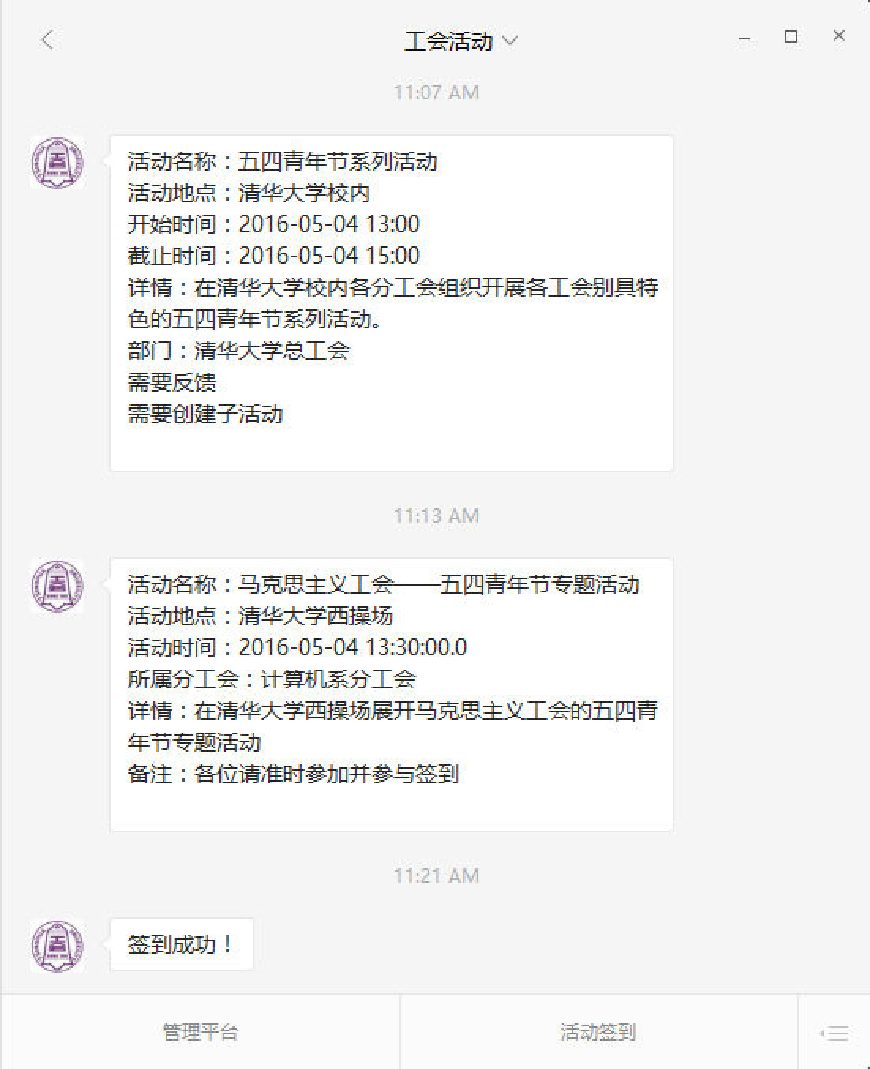
\includegraphics[width=0.8\textwidth]{shotPost.pdf}
  \caption{清华大学工会微信微平台界面}
  \label{fig:shotPost}
\end{figure}

当用户单击管理平台按钮之后,会进入到管理平台界面。通过管理平台,用户可以通过简单的操作对活动和子活动进行查看和管理,如图\ref{fig:shotWechatMenu}所示。

\begin{figure}[H]
  \centering
  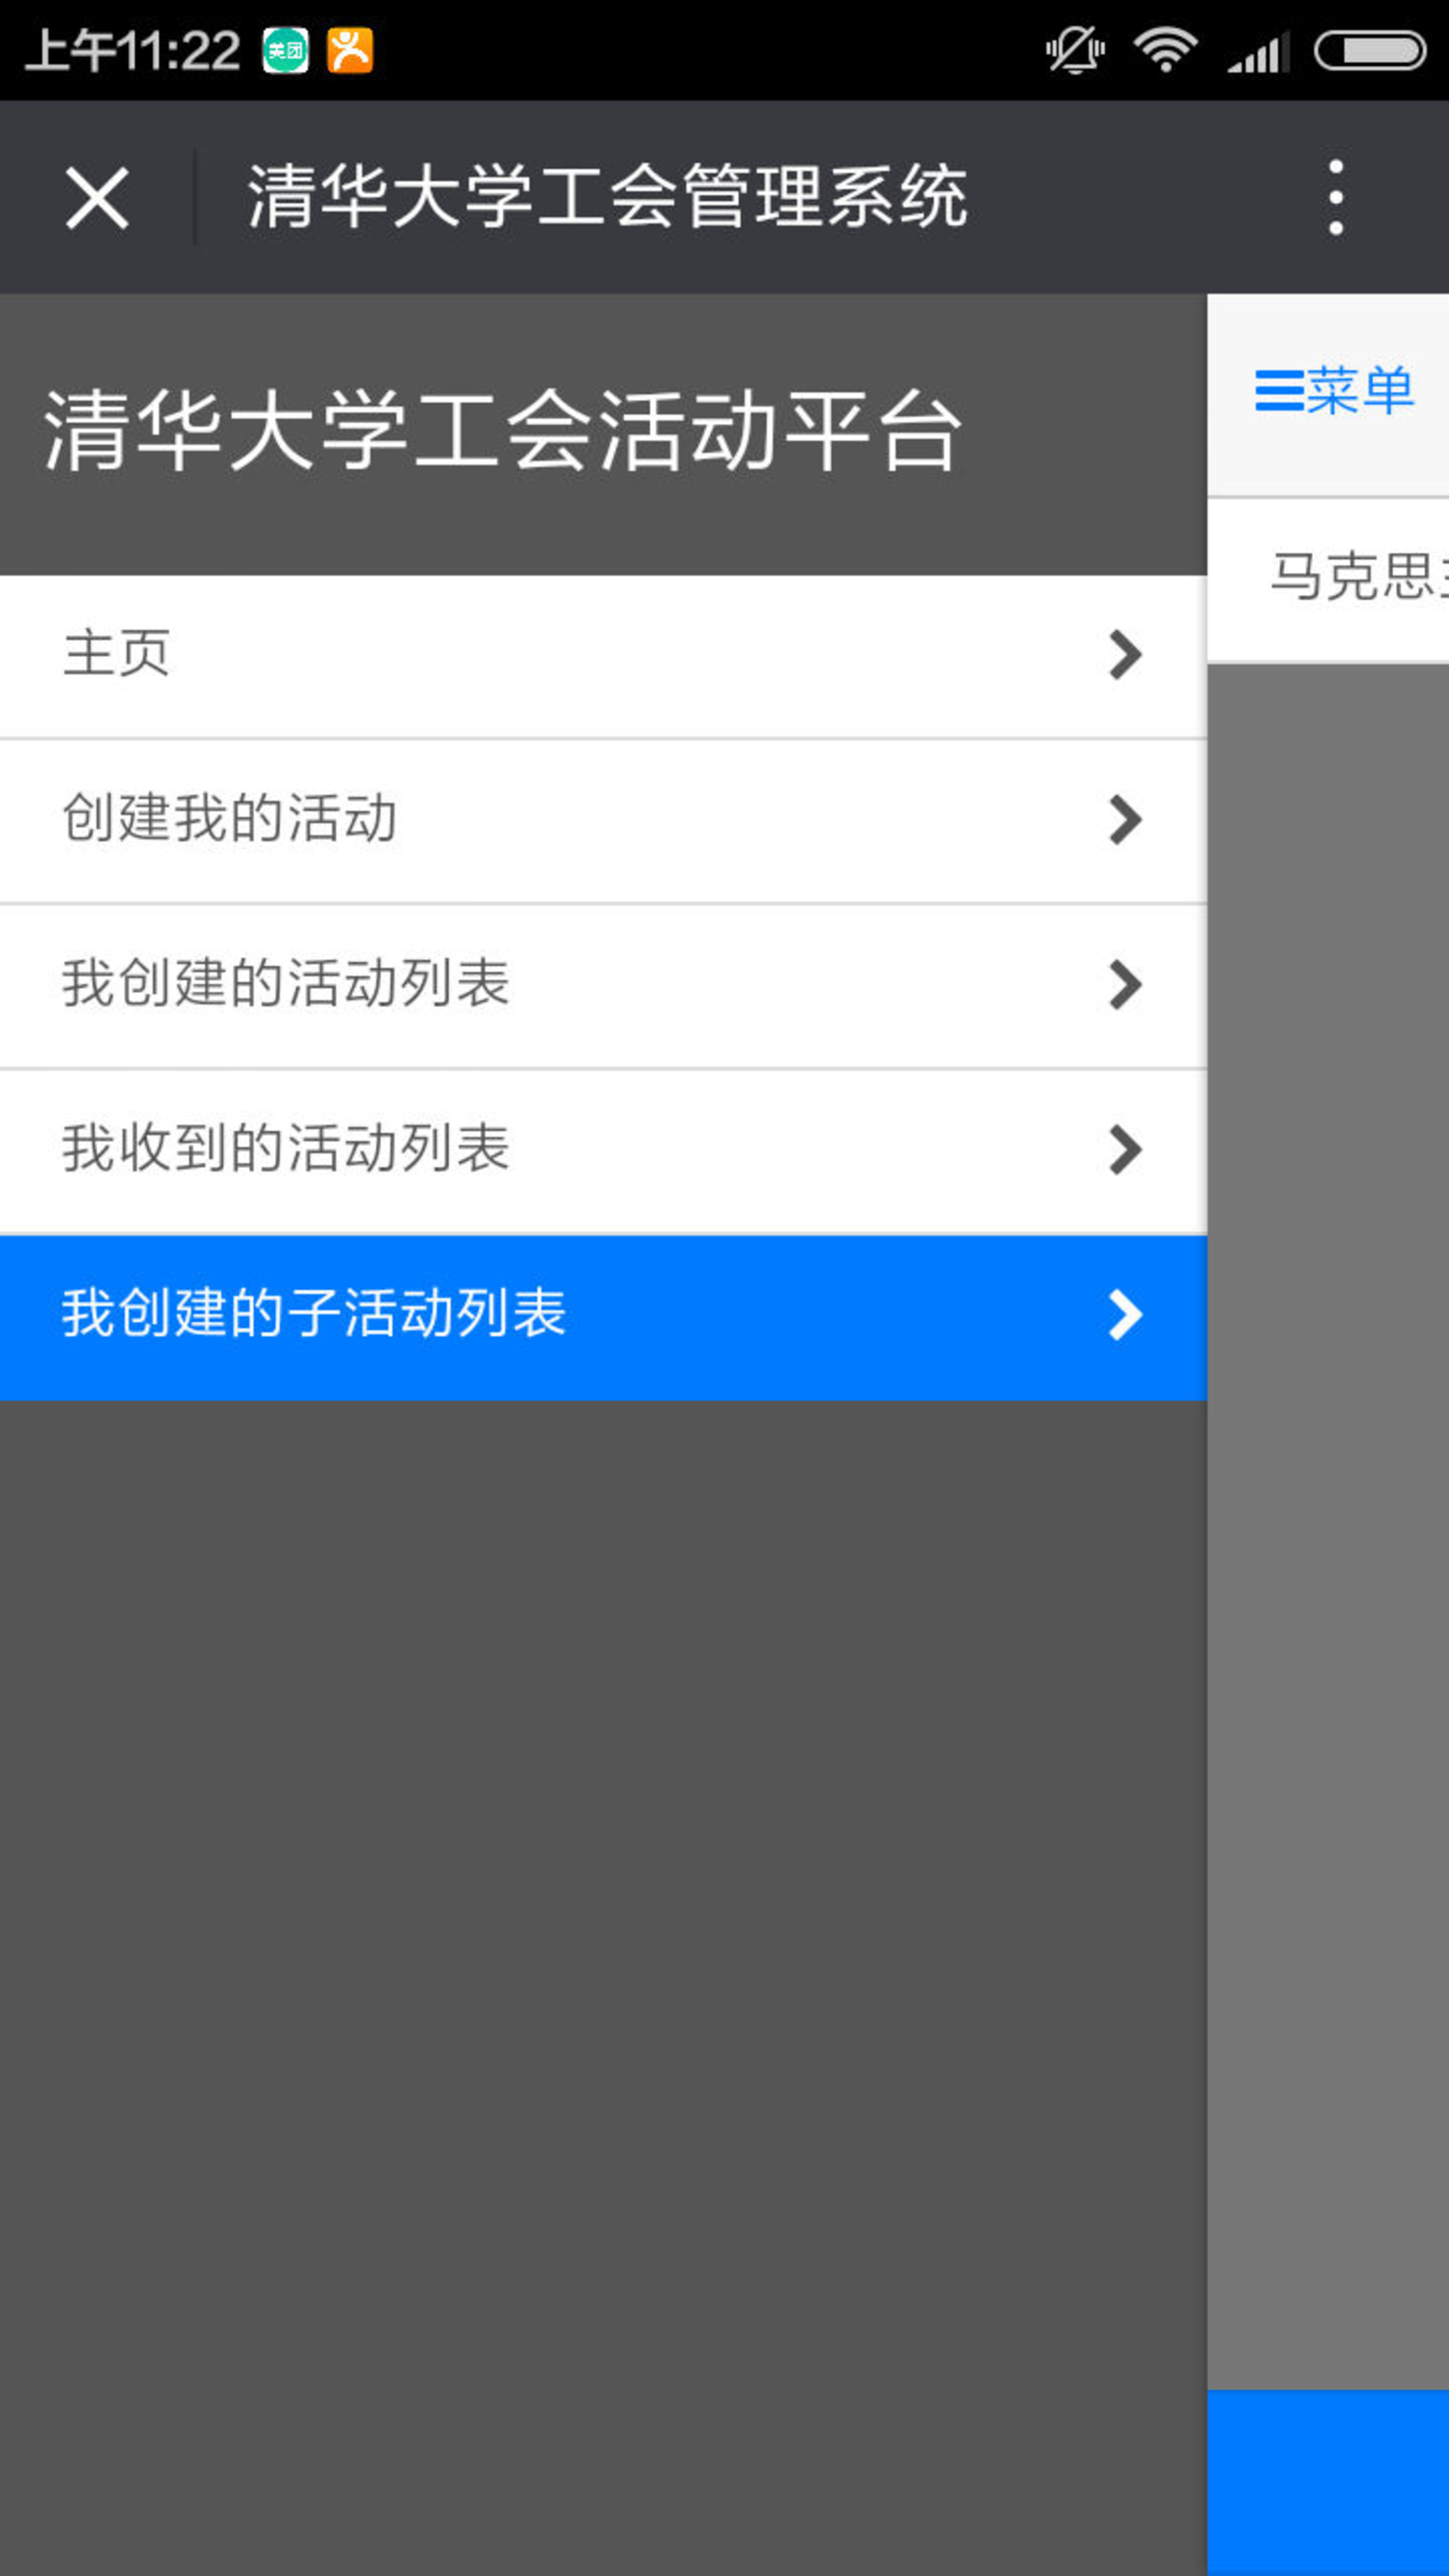
\includegraphics[width=0.5\textwidth]{shotWechatMenu.pdf}
  \caption{清华大学工会微信微平台管理平台界面}
  \label{fig:shotWechatMenu}
\end{figure}

进入收到的子活动,并选择相应的子活动栏目,就可以看到子活动的详细信息了(图\ref{fig:shotWechatDetail})。

\begin{figure}[H]
  \centering
  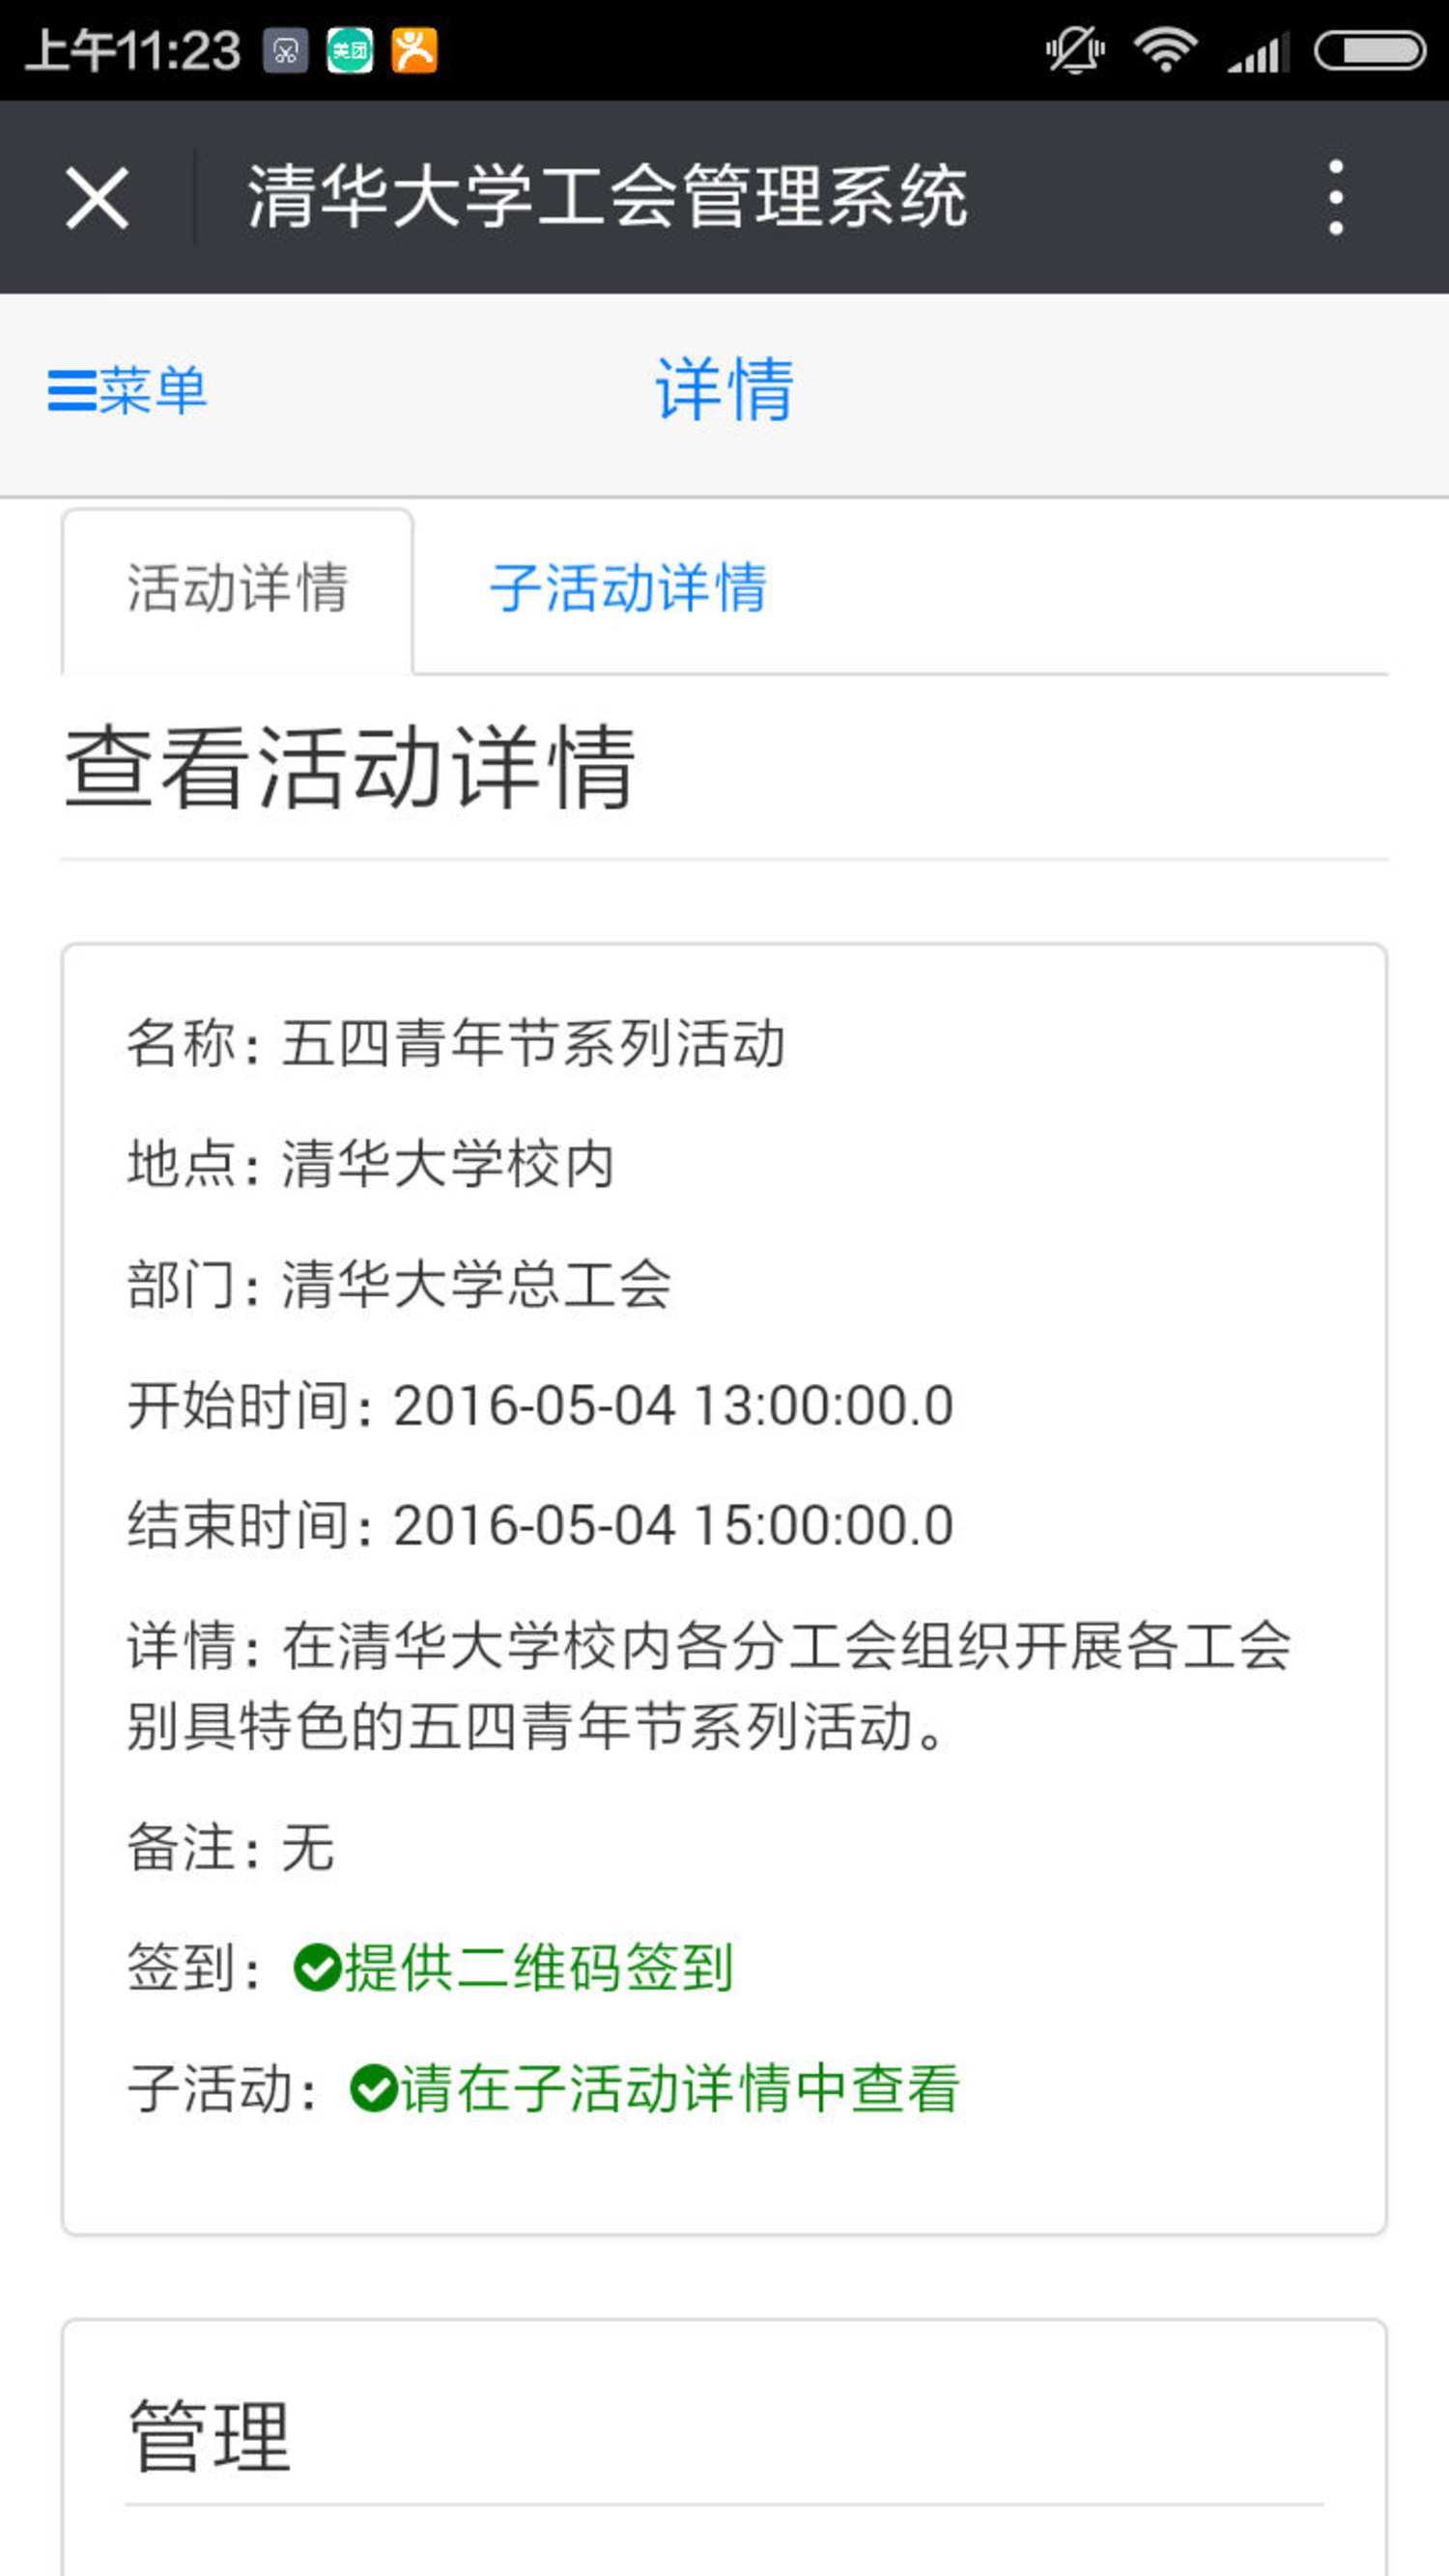
\includegraphics[width=0.5\textwidth]{shotWechatDetail.pdf}
  \caption{在工会微信管理平台查看子活动的详情}
  \label{fig:shotWechatDetail}
\end{figure}

除了能够查看子活动的详情以外,还能够在管理平台中对子活动进行方便的一键操作管理(图\ref{fig:shotWechatManage})。

\begin{figure}[H]
  \centering
  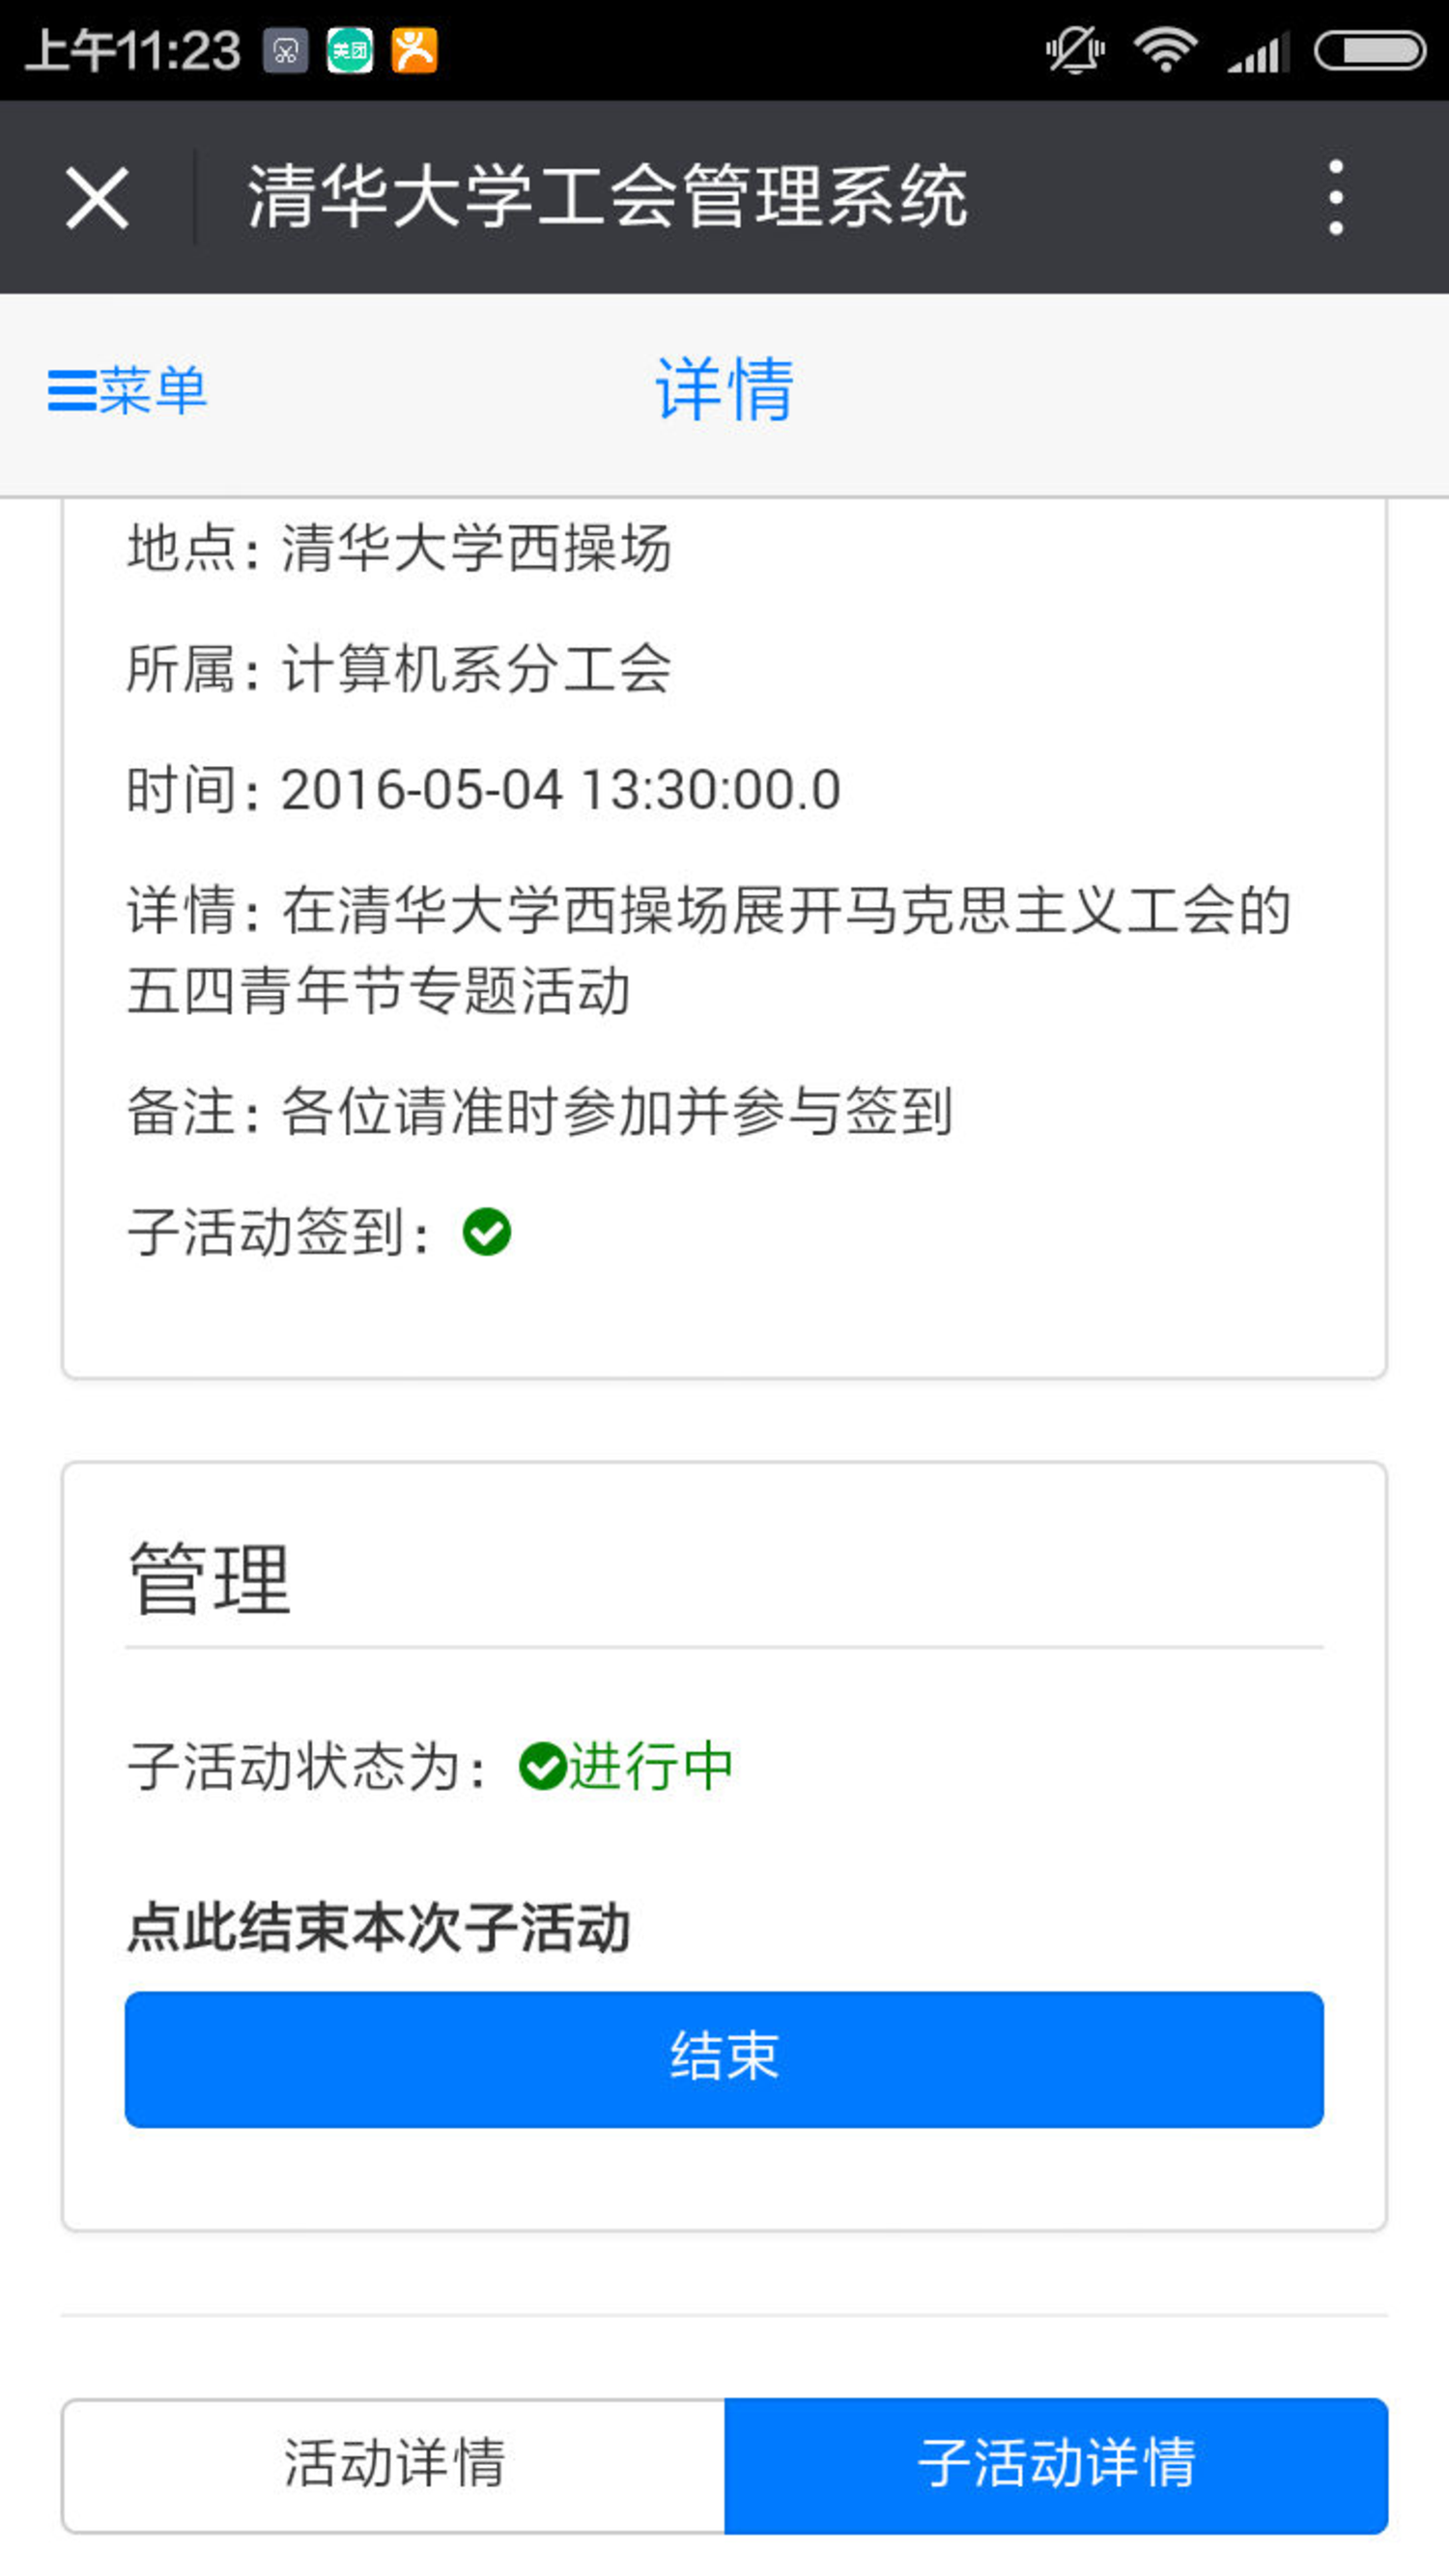
\includegraphics[width=0.5\textwidth]{shotWechatManage.pdf}
  \caption{在工会微信管理平台对子活动进行管理}
  \label{fig:shotWechatManage}
\end{figure}

\section{对比和评价}

在这一节中,我们将分别对清华大学工会管理系统的功能和性能进行定性和定量的评价。

\subsection{功能评价}

我们将清华大学工会管理系统与传统C/S行政系统、单纯B/S行政系统、基于HTTPS协议的B/S系统、基于微信公众号的C/S系统和基于移动应用的行政系统进行功能点对比。对比的功能点有:跨平台性,便携性,数据安全性,可用于行政系统目的,以及消息推送。评价结果见表\ref{table:compare}。


\begin{table}
  \centering
  \caption{不同平台系统的对比评价}
  \label{table:compare}
    \begin{tabular}{lccccc}
      \toprule
      系统 & 跨平台性 & 便携性能 & 数据安全 & 行政目的 & 消息推送 \\
      \midrule % $\surd$
      清华大学工会管理系统 		&$\surd$ &$\surd$ &$\surd$ &$\surd$ &$\surd$ \\
      传统C/S行政系统 			& & & &$\surd$ & \\
      单纯B/S行政系统 			&$\surd$ & & &$\surd$ & \\
      基于HTTPS协议的B/S系统 	&$\surd$ & &$\surd$ &$\surd$ & \\
      基于微信公众号的C/S系统 	&$\surd$ &$\surd$ & & &$\surd$ \\
      基于移动应用的行政系统 	& &$\surd$ & ? & $\surd$ & $\surd$\\
      \bottomrule
    \end{tabular}
\end{table}

从表\ref{table:compare}中可以看到,传统的C/S行政系统除了可以用于行政目的以外,已经无法跟上时代对行政系统的要求。在当今的多平台环境下,它已经逐渐被人们所淘汰。而单纯的B/S行政系统没有利用最近移动设备的发展给用户带来的便利,对于清华大学工会活动管理系统来说,无法进行及时的消息推送,同时数据的安全性也存在问题。虽然数据的安全问题可以通过使用HTTPS协议来保证,然而其缺乏移动设备上的支持和推送功能仍然使得它的应用范围受限。而基于微信公共号的新型C/S系统虽然可以充分利用到移动设备的便携性质,但是用于行政目的需要输入信息的时候,移动设备还是会不可避免地受到输入方式的限制,而且对文件的操作和处理存在很大的困难。对于微信公众号来说,信息的呈现形式也会受到很大的局限,只能借助微信平台的有限呈现模式来呈现信息。因此用单一的微信公众号作为行政系统的主体是不合适的。而基于移动应用的行政系统首先会要求用户安装相应的移动应用,并且移动应用不可避免地会遇到和微信公众号相同的问题。虽然移动应用可以通过对数据加密来满足数据的安全性,但是其存在的局限性仍然限制了它作为行政系统主体的能力。

可以看到,结合了B/S和C/S的优点,再加上对微信移动平台的充分运用,使得文中的清华大学工会管理系统不仅可以借助移动设备推送的能力满足工会活动通知的及时性,同时利用网页浏览器客户端使得信息的控制和管理更加高效灵活。

\subsection{性能评价}

通过对清华大学工会管理系统进行压力测试可以很好地描述出一个系统的性能。压力测试的后端运行环境如表\ref{table:hardware}所示。

\begin{table}
  \centering
  \caption{压力测试后端运行环境表}
  \label{table:hardware}
    \begin{tabular}{ll}
      \toprule
      项目 & 参数 \\
      \midrule % $\surd$
      计算机型号 & Lenovo Y510p \\
      CPU & Intel(R) Core i7-4700MQ @ 2.40 GHz \\
      硬盘 & SAMSUNG Spinpoint M8 ST1000LM024 @ 5400 RPM \\
      物理内存 & 8.00 GB \\
      操作系统 & Windows 10 Enterprise 64-bit \\
      Tomcat版本 & Apache Tomcat 7.0.55 \\
      MySQL版本 & mysql Ver 14.14 Distrib 5.6.20\\
      JAVA版本 & Java(TM) SE Runtime Environment (build 1.8.0\_73-b02)\\
      \bottomrule
    \end{tabular}
\end{table}


压力测试的内容是模拟不同数量的用户同时对系统进行1000次操作。测试的第一部分是将两个查询操作打包组成一组操作,并重复1000次,以此来测试平台在数据不进行修改的情况下的抗压能力。测试的第二部分是将一次插入操作和一次查询操作打包组成一组操作,并重复一千次,以此来考察当平台中的数据数量不断增大的时候,平台应对大量并发的操作时的相应时间。图\ref{fig:pressure}展示了压力测试的结果。

\begin{figure}[H]
  \centering
  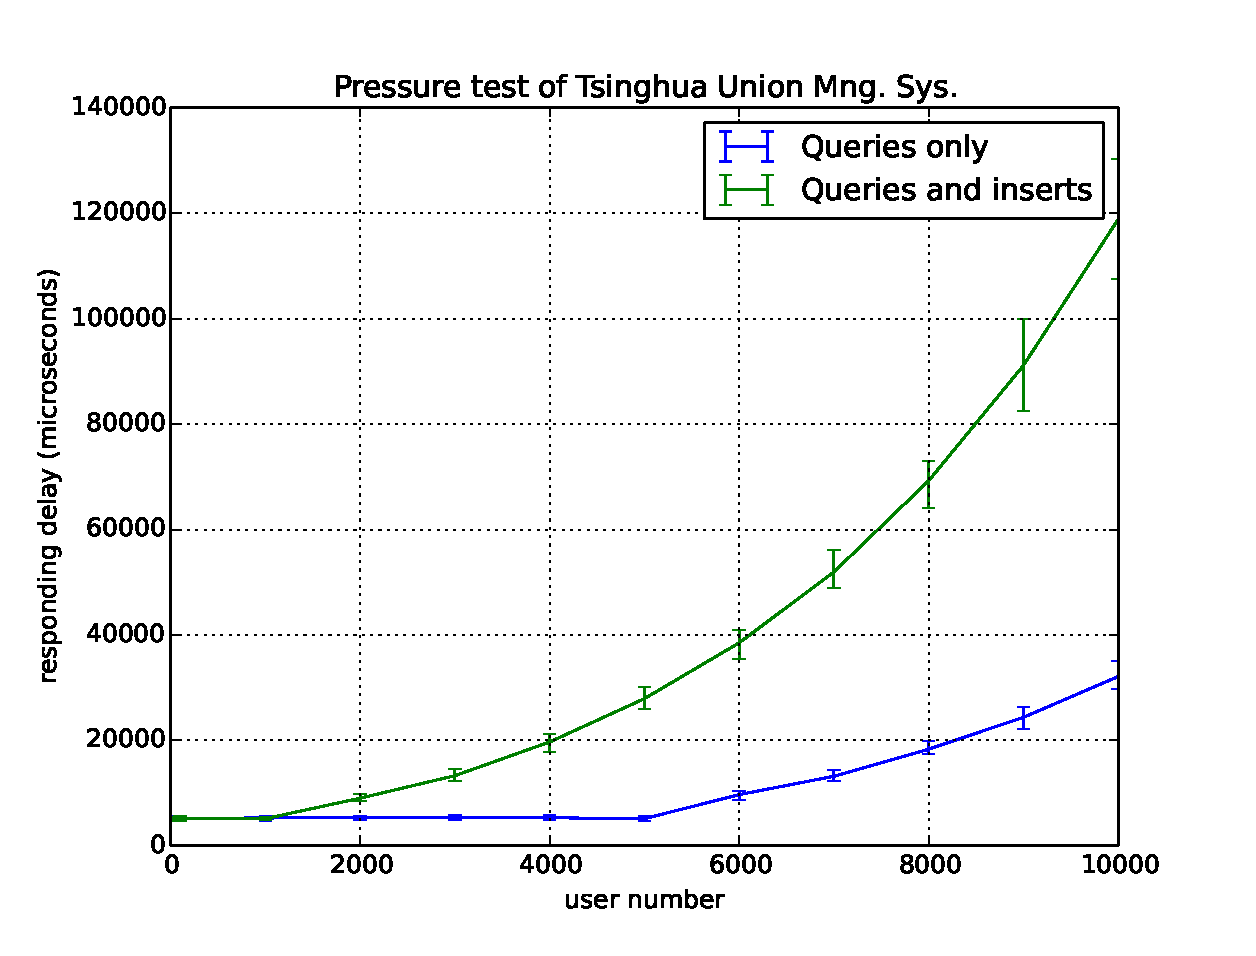
\includegraphics[width=0.8\textwidth]{pressureTest}
  \caption{压力测试结果图}
  \label{fig:pressure}
\end{figure}

图\ref{fig:pressure}中,横坐标为用户的数量,纵坐标为服务器的平均响应时间(单位:微秒)。从图中可以看到,在用户数量较少的时候,系统依然有5毫秒左右的相应延迟。这是由于建立HTTP连接和数据库连接会产生一定的时延。这个时延不可避免。另一方面,即使同时有10000个用户,每个用户连续发出1000次请求,系统依然能够在120毫秒左右给出响应。这充分说明了系统在架构设计的巧妙使得系统能够十分高效地运行。


\chapter{结论}

通过上述对B/S和C/S混合架构的行政管理系统的需求分析、架构设计、技术要点阐述以及样例系统的展示,本文展现了一套完整的B/S和新型C/S混合架构行政管理系统的设计开发方法。通过对系统进行一系列的评测和与同类系统的对比,我们展现了本系统的优势和亮点。

通过进一步完善本文中系统的鲁棒性,并扩展其功能和进行更多的测试,希望不远的未来文中的系统将能够正式地投入到清华大学工会中进行使用,能够真正服务于清华大学的师生工作当中,使得工会的活动和人员管理更为高效便捷。

希望本文能够为后续系统的开发提供架构和技术上的参考和支持。同时也希望随着越来越多的行政系统转移到互联网上,互联网办公能够成为为人们带来方便和福利的方式,切切实实地让人们感受到互联网科技带给人们的海阔天空。



%%% 其它部分
\backmatter

%% 本科生要这几个索引,研究生不要。选择性留下。
% 插图索引
\listoffigures
% 表格索引
\listoftables
% 公式索引
%\listofequations


%% 参考文献
% 注意:至少需要引用一篇参考文献,否则下面两行可能引起编译错误。
% 如果不需要参考文献,请将下面两行删除或注释掉。
\bibliographystyle{thuthesis}
\bibliography{ref/refs}

%% 致谢
% 如果使用声明扫描页,将可选参数指定为扫描后的 PDF 文件名,例如:
% \begin{ack}[scan-statement.pdf]
\begin{acknowledgement}
  衷心感谢导师张小平教授对本人的精心指导,信息中心刘乃佳学长在微信平台开发上为我提供的开放API支持,以及工会全体工作人员在需求分析上给我的帮助。他们的言传身教将使
  我终生受益。
\end{acknowledgement}


%% 附录
\begin{appendix}
%\input{data/appendix01}
\end{appendix}

%% 个人简历
%\include{data/resume}
\end{document}
